\documentclass[12pt,a4paper]{amsart}
% ukazi za delo s slovenscino -- izberi kodiranje, ki ti ustreza
\usepackage[slovene]{babel}
%\usepackage[cp1250]{inputenc}
\usepackage[T1]{fontenc}
\usepackage[utf8]{inputenc}
\usepackage{amsmath,amssymb,amsfonts}
\usepackage{url}
%\usepackage[normalem]{ulem}
\usepackage[dvipsnames,usenames]{color}
\usepackage{graphics}
\usepackage{pgf}
\usepackage{tikz}
\usepackage{graphicx}
\usepackage{bbm}
\usepackage{hyperref}
\hypersetup{
    colorlinks=true, %set true if you want colored links
    linktoc=all,     %set to all if you want both sections and subsections linked
    linkcolor=black,  %choose some color if you want links to stand out
}

\tikzstyle{block} = [rectangle, draw, 
    text width=8em, text centered, rounded corners, minimum height=4em]
\tikzstyle{line} = [draw, -latex]

% ne spreminjaj podatkov, ki vplivajo na obliko strani
\textwidth 15cm
\textheight 24cm
\oddsidemargin.5cm
\evensidemargin.5cm
\topmargin-5mm
\addtolength{\footskip}{10pt}
\pagestyle{plain}
\overfullrule=15pt % oznaci predlogo vrstico


% ukazi za matematicna okolja
\theoremstyle{definition} % tekst napisan pokoncno
\newtheorem{definicija}{Definicija}[section]
\newtheorem{primer}[definicija]{Primer}
\newtheorem{opomba}[definicija]{Opomba}

\renewcommand\endprimer{\hfill$\diamondsuit$}


\theoremstyle{plain} % tekst napisan posevno
\newtheorem{lema}[definicija]{Lema}
\newtheorem{izrek}[definicija]{Izrek}
\newtheorem{trditev}[definicija]{Trditev}
\newtheorem{posledica}[definicija]{Posledica}
\newtheorem{zgled}[definicija]{Zgled}
\newtheorem{hipoteza}[definicija]{Hipoteza}


% za stevilske mnozice uporabi naslednje simbole
\newcommand{\R}{\mathbb R}
\newcommand{\N}{\mathbb N}
\newcommand{\Z}{\mathbb Z}
\newcommand{\C}{\mathbb C}
\newcommand{\Q}{\mathbb Q}

% ukaz za slovarsko geslo
\newlength{\odstavek}
\setlength{\odstavek}{\parindent}
\newcommand{\geslo}[2]{\noindent\textbf{#1}\hspace*{3mm}\hangindent=\parindent\hangafter=1 #2}

% naslednje ukaze ustrezno popravi
\newcommand{\program}{Finančna matematika} % ime studijskega programa: Matematika/Finan"cna matematika
\newcommand{\imeavtorja}{Jure Babnik} % ime avtorja
\newcommand{\imementorja}{~prof.~dr. Tomaž Košir} % akademski naziv in ime mentorja
\newcommand{\naslovdela}{Finančni instrumenti in razvoj upravljanja s tveganjem}
\newcommand{\letnica}{2021} %letnica diplome


% vstavi svoje definicije ...




\begin{document}

% od tod do povzetka ne spreminjaj nicesar
\thispagestyle{empty}
\noindent{\large
UNIVERZA V LJUBLJANI\\[1mm]
FAKULTETA ZA MATEMATIKO IN FIZIKO\\[5mm]
\program\ -- 1.~stopnja}
\vfill

\begin{center}{\large
\imeavtorja\\[2mm]
{\bf \naslovdela}\\[10mm]
Delo diplomskega seminarja\\[1cm]
Mentor: \imementorja}
\end{center}
\vfill

\noindent{\large
Ljubljana, \letnica}
\pagebreak

\thispagestyle{empty}
\tableofcontents
\pagebreak

\thispagestyle{empty}
\begin{center}
{\bf \naslovdela}\\[3mm]
{\sc Povzetek}
\end{center}
% tekst povzetka v slovenscini
Podjetja in finančne inštitucije se pri poslovanju že od nekdaj srečujejo z različnimi oblikami 
tveganja. Pomembno je tveganje razumeti, poznati različne oblike tveganja, ter znati 
obvladovati tveganje. Za to je potrebno poznati različne finančne instrumente, ki so na voljo 
na trgu, tudi preproste in bolj zapletene izvedene finančne instrumente. Obstajajo različni 
modeli vrednotenja naložb in ocenjevanja tveganja, kot so CAPM model, Black-Scholesova 
formula, RiskMetrics, katere pokriva tudi moja diplomska naloga. Poznamo različne mere 
tveganja, namenjene vrednotenju tveganja in ugotavljanju primerne količine kapiala, potrebne 
za kritje. Da lahko trg nemoteno deluje, skrbijo različni regulatorni organi in sistemi regulacij. V 
primeru površnega upravljanja s tveganjem in neučinkovitih regulacij pa lahko pride do hudih 
posledic, kot je globalna finančna kriza.
\vfill
\begin{center}
{\bf Financial Instruments and Evolution of Risk Management}\\[3mm] % prevod slovenskega naslova dela 
{\sc Abstract}
\end{center}
% tekst povzetka v anglescini
Companies and financial institutions are constantly facing various risk that come in all shapes 
and sizes. It is essential not only to understand them, but also be able to manage the risk. 
Knowing different financial instruments is imperative, especially with such a broad spectrum of 
existing instruments, including simple and more complex derivatives. There are many models 
for evaluating investments and measuring risks, such as CAPM model, Black-Scholes model and 
RiskMetrics, all of which are covered in this paper. Risk measures are used for evaluating risks 
and calculating the amount of capital required to cover potential losses. In order for the market 
to function seemlessly, different regulatory systems are in place, enforced by competent 
regulatory authorities. Negligent risk assessment and management, along with inefficient 
regulations can lead to catastrophic consequences, such as global financial crisis.


%POPRAVI !!!!!!!!!!!!!!!!!!!!!!!!!!!!!!!!!!!!!!!!!!!!!!!!!!!!!!!!!!!!!!!!!!!!!!!!!!!!!!!!!!!!!!!!!!!!!!!!!!!!!!!!!!!!!!!!!!!!!!!!!!!!!!!!!!!!!!!!!!!!!!!!!!!!!!!
\vfill\noindent
{\bf Math. Subj. Class. (2010):} navedite vsaj eno klasifikacijsko oznako -- 
        dostopne so na \url{www.ams.org/mathscinet/msc/msc2010.html}  \\[1mm]  
{\bf Ključne besede:} Upravljanje s tveganjem, finančni instrumenti  \\[1mm]  
{\bf Keywords:} Risk management, financial instruments
\pagebreak



% tu se zacne tekst seminarja
\section{Uvod}
%Na za"cetku prvega poglavja/razdelka (ali v samostojnem razdelku z naslovom Uvod) napi"site 
%kratek zgodovinski in matemati"cni uvod. Pojasnite motivacijo za problem, kje nastopa, kje 
%vse je bil obravnavan. Na koncu opi"site tudi organizacijo dela -- kaj je v kak"snem razdelku.
%
%"Ce se uvod naravno nadaljuje v besedilo prvega poglavja, lahko nadaljujete z besedilom v istem 
%razdelku, sicer za"cnete novega. Na za"cetku vsakega razdelka/podraz\-delka povete, "cemu se 
%bomo posvetili v nadaljevanju. Pri pisanju uporabljajte ukaze za matemati"cna okolja, med 
%formalnimi enotami dodajte vezni razlagalni tekst.


\subsection{Motivacija}
Upravljanje s tveganjem je zelo pomemben del poslovanja. Tveganje je namreč prisotno pri 
praktično vsakem poslu, zato ga je potrebno obvladovati in se tako izogniti neprijetnim
posledicam, ali pa jih vsaj kar se da omiliti. V resnici so tveganju izpostavljena vsa podjetja, 
finančne institucije, pa tudi posamezniki, prihaja pa v najrazličnejših oblikah in povzroča posledice
različnih oblik in velikosti. Skozi čas se je na trgu pojavilo mnogo novosti. Novi instrumenti so omogočali drugačne 
donose, hkrati pa so predstavljali tudi nova tveganja. Zato je pomembno, da so se hkrati razvile 
tudi nove metode prepoznavanja in upravljanja s tveganjem.

\subsection{Tveganje} Najprej je potrebno razumeti, kaj sploh je \textbf{finančno tveganje}. Gre za 
kakršno koli možnost izgube denarja ali sredstev pri katerem koli poslu. Nastane kot posledica
različnih dejavnikov, ki so lahko bodisi endogeni (notranji) bodisi eksogeni (zunanji). Poznamo 
pet glavnih vrst tveganja:
\begin{itemize}
  \item \textbf{Čisto tveganje}: to je neobvladljivo tveganje, ki ima le dva možna izida: brez
	izgube ali pa popolna izguba.
  \item \textbf{Tržno tveganje}: nastane kot posledica tržnih sprememb. Sem spadajo spremembe
	obrestne mere, spremembe cen blaga, menjalnih tečajev, donosnosti sredstev, itd.
  \item \textbf{Tveganje neplačila}: gre za tveganje, da dolžnik ne bo poravnal dolga. S to obliko
	tveganja se ne srečujejo le posojilodajalci, temveč vsi upniki.
  \item \textbf{Operativno tveganje}: pri opravljanju vsakodnevnih dejavnosti se podjetja srečujejo
	s to obliko tveganja. Sem sodijo razne okvare računalniških sistemov, napake zaposlenih, 
	prevare, itd.
  \item \textbf{Likvidnostno tveganje}: možnost primanjkljaja likvidnih sredstev za poravnavo
	kratkoročnih obveznosti.
\end{itemize}

\subsection{Upravljanje s tveganjem}
Razvidno že iz samega imena, izraz \textbf{upravljanje s tveganjem} označuje postopek identifikacije, 
analize, in nato obvladovanja tveganja. V praksi se tveganja ne da povsem odpraviti, je pa 
mogoče tveganje zmanjšati, zato je glavni cilj upravljanja s tveganjem kar se da omejiti tveganje. 
Poleg tega lahko vplivamo tudi na posledice neugodnih razmer, zato jih želimo z ustreznimi 
strategijami kar se da omiliti. Pogosto se uporabljajo najrazličnejši finančni instrumenti, kot so npr.
opcije, terminske pogodbe, pa tudi bolj zapleteni instrumenti, in pa različne strategije. 
Najosnovnejša strategija je diverzifikacija portfelja, ali kot pravijo, ">ne nosite vseh jajc v eni 
košari"<.


\subsection{Struktura naloge}
V uvodnem delu razložimo pojma \textit{tveganje} in \textit{upravljanje s tveganjem}. Celotna 
naloga je urejena kar se da kronološko. Sprehodimo se skozi začetke upravljanja s tveganjem in
si nato pogledamo nekaj preprostih instrumentov in strategij. Sledijo prvi modeli, povezani z 
finančnimi instrumenti, skupaj z njihovimi predpostavkami in pomanjkljivostmi. Nato si pogledamo 
modela RiskMetrics in CreditMetrics, zraven pa si pogledamo tudi nekaj mer tveganja in razložimo 
pojem \textit{koherentne mere tveganja}. Nato si pogledamo regulacije. Sledijo novejši in bolj 
zapleteni izvedeni finančni instrumenti, zaključimo pa s finančno krizo leta 2008 in povezavo z 
napakami oz. površnostmi na področju finančnih instrumentov in obvladovanja tveganja.

\section{Začetki upravljanja s tveganjem}
%https://www.ventivtech.com/blog/a-brief-summary-of-the-long-history-of-risk-management			$DONE
Zgodovinarji verjamejo, da začetki upravljanja s tveganjem izhajajo iz iger na srečo. Koncepti
zavarovanja v primeru nezgodnih situacij segajo celo v čase Rimljanov. V 18. stoletju so se pojavila 
prva življenska zavarovanja, upravljanje s tveganjem kot ga poznamo danes, pa se je v resnici 
pojavilo v času po drugi svetovni vojni, z rojstvom moderne finančne teorije. Do danes se je 
pogled na tveganje precej spremenil, zato pa so tudi pristopi obvladovanja tveganja drugačni.

\subsection{Brownovo gibanje}
%https://en.wikipedia.org/wiki/Louis_Bachelier										$DONE
%https://en.wikipedia.org/wiki/Brownian_motion										$DONE
Francoski matematik Louis Bachelier je leta 1900 objavil raziskovalno delo, v katerem je opisoval 
proces gibanja cene vrednostnega papirja. Delo takrat ni bilo dobro 
sprejeto, saj je bilo takrat področje financ matematikom precej tuje, zato kljub odlični vsebini 
delo ni bilo posebej odlikovano. V delu je opisoval gibanje, ki ga danes poznamo 
pod imenom \textbf{Brownovo gibanje}. Pojav opisuje gibanje delcev v kapljevini. Imenuje se po botaniku
Robertu Brownu, ki je ta pojav prvi opisal leta 1827, kasneje pa je Albert Einstein leta 1905 
objavil delo, v katerem modelira gibanje delca cvetnega prahu med molekulami vode. Leta 1908
je to utemeljil francoski fizik Jean Baptiste Perrin in zato kasneje prejel tudi Nobelovo nagrado.

%Quote iz tle https://www.cambridge.org/core/journals/british-journal-for-the-history-of-science/article/abs/case-of-brownian-motion-a-note-on-bacheliers-contribution/EFCA1863B23ACF2339CCF9E6C26EB659
																	%DONE
Odkritje pojava je služilo kot dokaz obstoja atomov in molekul. Kako pa je to povezano z vrednostnimi
papirji? Bistvo je v tem, da je gibanje delca nemogoče napovedati. Model, ki bi upošteval vsako 
molekulo in deterministično podal pot delca, ne obstaja. Gibanje delca je povsem naključno. 
Bachelier je slednje predpostavil tudi za cene vrednostnih papirjev, saj tudi na njihovo vrednost
vpliva ogromno dejavnikov, tako kot na gibanje delca cvetnega prahu vplivajo ostale molekule 
vode.


\begin{quotation}
   	">V danem trenutku trg verjame, da je cena pravična, in ne pričakuje ne dviga, ne padca cene.
	Najverjetnejša cena je prava tržna cena. Če bi trg mislil drugače, bi bila že trenutna cena višja ali
	nižja. Matematično upanje špekulanta je vedno enako $0$."<
\end{quotation}

Ideja je sledeča: nihče
ne pozna in ne more predvideti gibanja cene instrumenta. Če bi se cena instrumenta kadar koli 
gibala po predvidljivi poti, bi bilo gibanje mogoče predvideti. Ker je gibanje mogoče predvideti, ga
bo nek tržni udeleženec predvidel. V trenutku, ko izkoristi svoje informacije, z nakupom oz. prodajo
vpliva na celoten trg in spremeni gibanje cene, s tem pa uniči predvidljivo gibanje.


\subsection{Začetki}
%https://en.wikipedia.org/wiki/The_Journal_of_Finance									%DONE
%https://en.wikipedia.org/wiki/American_Finance_Association								%DONE
Leta 1939 je bila ustanovljena ameriška finančna zveza (angl. \textit{American Finance Association}).
Glavni cilji zveze so ozaveščanje javnosti o finančnih problemih, zagotavljanje platform za izmenjavo 
informacij, spodbujajo pa tudi izobraževanje na temo financ na višjih šolah in univerzah. Leta
1942 je prvič izšel njihov dnevnik z naslovom Ameriške finance (angl. \textit{American Finance}),
ki pa se je leta 1946 preimenoval v Dnevnik financ (angl. \textit{Journal of Finance}) in pod
tem imenom izhaja še danes. V njem so objavljene raziskave iz vseh glavnih področij financ.
Izhaja šestkrat letno (torej vsak drugi mesec), najboljši članki pa so vsako leto nominirani za 
Brattlovo in Smith Breedenovo nagrado. Prva je podeljena najboljšemu članku s področja 
poslovnih financ, Smith Breedenova pa najboljšemu članku s katerega koli drugega finančnega
področja.

%https://www.aria.org/about-aria/												%DONE
%https://en.wikipedia.org/wiki/Journal_of_Risk_and_Insurance								%DONE
Poleg tega je bila leta 1932 ustanovljena ameriška zveza za tveganje in zavarovanje (angl.
\textit{American Risk and Insurance Association, ARIA}). Ukvarja se z izobraževanjem in 
podporo profesionalcev in študentov področja zavarovanja in upravljanja s tveganjem. Od
leta 1933 (do danes) vsako četrtletje izide njihov Dnevnik tveganja in zavarovanja (angl. 
\textit{Journal of  Risk and Insurance}), ki je bil vmes poznan tudi pod nekaterimi malce 
drugačnimi imeni, trenutno ime pa je dobil šele leta 1964. Pomemben je zato, ker so bili v 
njem objavljeni prvi članki na temo tveganja in zavarovanja.


\subsection{Moderno upravljanje s tveganjem}
Upravljanje s tvegnjem je relativno nova korporacijska funkcija. Začetki modernega upravljanja
s tveganjem segajo nekje v šestdeseta leta prejšnjega stoletja. Do danes se je že precej razvilo
in spremenilo. Morda najbolj opazna sprememba je manjša odvisnost od tržnega zavarovanja,
ki danes služi bolj ali manj le kot dodatek k večim različnim komponentam obvladovanja tveganja.
Vse bolj pomembne so sledeče aktivnosti:
\begin{itemize}
  \item \textbf{Samozaščitne aktivnosti}: so vse tiste aktivnosti, ki vplivajo na verjetnost, da bi
	prišlo do izgub, ali pa na količino izgub, do katerih bi zaradi tega vzroka prišlo (npr. 
	najrazličnejši previdnostni ukrepi)
  \item \textbf{Samozavarovalne aktivnosti}: so vse tiste aktivnosti, ki ustvarjajo relativno 
	likvidne rezerve, ki bi se uporabile za kritje izgub v primeru kakšne nesreče ali poslabšanju
	razmer na trgu.
\end{itemize}

V sedemdesetih letih je upravljanje s tveganjem doživelo največji razvoj, skoraj da pravo 
revolucijo. Postalo je prioriteta za vse inštitucije, ki so bile izpostavljene tveganju, povezanim
z obrestnimi merami, deviznimi tečaji, cenami surovin, ipd. Bilo je zelo pomembno, saj so bile
cene omenjenega blaga v tem časovnem obdobju zelo nestanovitne. Da bi se zavarovali, so
začeli uporabljati \textbf{izvedene finančne instrumente} (angl. \textit{derivatives}). Bili so 
odlična izbira, saj so ponujali malo bolj specifična in raznolika izplačila, ki so se med seboj 
razlikovala glede na tržne pogoje. Danes so najbolj poznani izvedeni finančni instrumenti opcije,
terminske pogodbe na blago ali obrestno mero, ter zamenjave.

Zaradi obstoja bolj zapletenih instrumetnov je bilo vse težje oceniti tveganja, katerim je bilo neko
podjetje izpostavljeno, poleg tega pa so se pojavila tudi nova tveganja, ki jih je bilo vse težje
sploh prepoznati oz. nadzorovati. Kot odgovor na to se je ">definicija"< upravljanja s tveganjem
malce spremenila.

Odločitve so začenjali sprejemati po drugačnem kriteriju. Pred tem so se osredotočali na vsako 
tveganje oz. na vsako situacijo posebej. Vsako odločitev so sprejemali na podlagi tega, kako dobro
krije določeno tveganje, kar pa je postalo kar precej zapleteno. Zato so poiskali drugačen pristop.
Odločitve so začeli sprejemati na podlagi generalnega vpliva na portfelj v različnih potencialnih
stanjih ekonomije v prihodnosti. To je nekako posplošilo definicijo upravljanja s tveganjem.

\subsection{CBOE}
Sledilo je obdobje hitrega razvoja na področju financ. Kot že omenjeno, so se na trgu pojavili mnogi novi izvedeni
finančni instrumenti. Vsak izmed njih je imel drugačna izplačila, hkrati pa drugačna tveganja. 
Leta 1973  je bila 
ustanovljena Čikaška borza za opcijske pogodbe (angl. \textit{Chicago Board Options
Exchange, CBOE}). Vzporedno so odprli tudi klirinško hišo. V tem obdobju je trg doživel velik
razvoj. Rast in razvoj trga opcij se je drastično povečal po tem, ko je CBOE standardizirala 
pogodbe in razvila sekundarne trge potrebne, da je na trgu dovolj likvidnih sredstev za 
tržno učinkovitost. Kasneje, v osemdesetih in devetdesetih letih, je implementacija teh 
produktov tržne udeležence ozaveščala o tveganju, s katerim se srečujejo pri 
vsakodnevnem trgovanju.

\section{Preprosti instrumetni in strategije}
Z uporabo preprostih istrumentov, kot so opcije in terminske pogodbe, lahko oblikujemo 
osnovne strategije, ki služijo kot zavarovanje pred izgubami. Te strategije imajo seveda 
tudi slabo stran. V zameno za zavarovanje pred velikimi izgubami moramo po navadi 
nekaj plačati, ali pa se odpovedati tudi velikim dobičkom. Poglejmo si nekaj preprostih 
izvedenih finančnih instrumentov. Pomembno je razumeti njihova izplačila, ki sicer niso 
preveč zapletena, a vseeno niso tako direktna kot npr. izplačila obveznice ali delnice. 

\subsection{Terminske pogodbe}
%https://www.investopedia.com/terms/f/futurescontract.asp							%DONE
Pogodbo, ki določa nakup ali prodajo točno določenega osnovnega sredstva (angl. 
\textit{underlying}) ob točno določenem času v prihodnosti, imenujemo \textbf{terminska 
pogodba} (angl. \textit{future contract}, ali na kratko \textit{future}). V njej so natančno 
določeni najrazličnejši podatki o blagu ali instrumentu (da obe strani natanko vesta, kaj 
kupujeta oz. prodajata), izvršilni ceni, času izvršitve, itd. V praksi se večina pogodb sploh ne izvrši, 
saj investitorji instrument uporabljajo kot investicijo in ne za dejanski nakup ali prodajo blaga. 
Zato svojo pozicijo po navadi predčasno zaprejo.

Naj bo $K$ izvršilna cena, $T$ čas izvršitve terminske pogodbe, 
$S_t$ cena osnovnega sredstva v času $t$ in $D(t_1, t_2)$ 
diskontni faktor za časovno obdobje $[t_1, t_2]$. Potem je vrednost $V_t$ pogodbe 
v času $t$ enaka:
$$V_t = S_t - KD(t, T),$$
kar mora za $t=0$ seveda biti enako $0$, saj bi v nasprotnem primeru imeli možnost 
arbitraže. 

Terminska pogodba dovoli nakup osnovnega sredstva ob kasnejšem času za v naprej 
dogovorjeno ceno. V obdobju, ko so cene nestanovitne, je to zelo koristno. Recimo, 
da se dogovorimo za nakup $x$ steklenic vode po ceni $1$ evro na steklenico (kar naj 
bo tudi trenutna cena) čez pol leta. Če cena naraste na $1,10$ evra, potem smo 
privarčevali $10$ centov na steklenico. Če pa cena pade na $0,90$ evra, pa bi jih 
lahko na prostem trgu kupili za $10$ centov na steklenico ceneje in smo ta denar 
zapravili. Pogodba je zelo koristna, saj nas zaščiti pred dvigom cene, čeprav nam lahko 
prinese tudi izgube. Za dolgo stran pogodbe je izkupiček v obeh scenarijih 
ravno nasproten. 

\subsection{Zamenjave}
%https://www.investopedia.com/terms/s/swap.asp									%DONE
Pogodba med dvema stranema, ki se dogovorita o zamenjavi določenih denarnih tokov ali obveznosti, 
se imenuje zamenjava (angl. \textit{swap}). Poznamo različne tipe zamenjav, najpreprostejše 
in najpogostejše so zamenjave obrestnih mer. Na voljo so bolj ali manj izključno na prostem 
trgu. Uporabljajo se predvsem za upravljanje s tveganjem oz. zavarovanje, v primeru ko 
npr. pričakujemo porast obrestne mere, se lahko dogovorimo za zamenjavo obresnte mere. 

Recimo, da si podjetje izposodi milijon evrov, nato pa naslednjih pet let plačuje 
obresti po tržni obrestni meri (EURIBOR). Recimo, da ob sklenitvi ta obresnta mera 
znaša $1\%$. Podjetje pričakuje, da se bo močno povišala v prihodnjih petih 
letih, zato se dogovori za zamenjavo obrestne mere z neko finančno inštitucijo, 
dogovorijo pa se za fiksno obrestno mero $2\%$. Poglejmo si tri možne scenarije: 
\begin{itemize}
  \item Recimo, da v prvem letu EURIBOR ostane nespremenjen. Podjetje je torej 
	dolžno plačati dogovorjena $2\%$ finančni inštituciji, ki pa mora plačati le $1\%$ 
	obresti na posojilo podjetja. 
	Podjetje z zamenjavo torej izgubi $1\%$, ali $10.000$ evrov. 
  \item Recimo, da v tretjem letu tržna obresna mera naraste na $2\%$. Podjetje je 
	spet dolžno plačati dogovorjena $2\%$, enako kot finančna inštitucija. 
	Podjetje v tem primeru nima ne profita ne izgube. 
  \item V zadnjem letu tržna obrestna mera močno naraste, recimo na $4\%$. Podjetje 
	kot vedno plača $2\%$, finančna inštitucija pa tokrat $4\%$, zato podjetje v 
	tem letu z dogovorom zabeleži $2\%$ oz. $20.000$ evrov profita.
\end{itemize}

Denarni tokovi obeh strani pogodbe so torej zamenjani.
Lahko vidimo, da se tovrstna zamenjava (z vidika podjetja) izkaže za dobro naložbo v primeru, ko 
obrestne mere dovolj narastejo. Če ostanejo nespremenjene ali celo padejo, 
potem si podjetje naredi izgubo. Zamenjave so zelo uporabne, saj se podjetje 
lahko zaščiti pred povečanjem obrestne mere. Pogosto so podjetja pripravljena 
sprejeti manjše izgube, če le to pomeni zavarovanje pred potencialnimi velikimi 
izgubami, ki bi lahko močno ogrozile njihovo poslovanje ali celo preživetje.

Omenimo še, da v praksi obe strani dobesedno ne plačujeta obresti druga za drugo. Pri 
zamenjavah se ob vsakem roku 
plačil obresti načeloma le poravna razlika obeh plačil . 


\subsection{Opcije}
%https://en.wikipedia.org/wiki/Option_(finance)									%DONE
%https://www.investopedia.com/terms/o/option.asp								%DONE

Podobno kot terminske pogodbe, so tudi opcije (angl. \textit{options}) pogodbe, ki 
imajo točno določeno ročnost, osnovno sredstvo, ceno, itd. Glavna razlika med opcijo 
in terminsko pogodbo je ta, da ima kupec opcije ob dospetju \textbf{pravico do nakupa}
osnovnega sredstva, kupec terminske pogodbe pa \textbf{mora} osnovno sredstvo kupiti. 
Seveda to predstavlja veliko prednost za kupca opcije. 

Imetnik nakupne opcije se bo odločil za nakup sredstva v primeru, ko je v času dospetja 
trenutna cena \textbf{višja od dogovorjene}, v nasprotem primeru pa ne izvrši. Za imetnika 
prodajne opcije velja ravno obratno; za prodajo se bo odločil v primeru, ko je v času 
dospetja trenutna cena \textbf{nižja} od dogovorjene, sicer pa opcije ne izvrši. 
Izplačila obeh opcij (ob času odspetja $T$) lahko torej zapišemo na sledeč način:
$$C_T = max(S_T - K, 0) \text{ in}$$ 
$$P_T = max(K - S_T, 0),$$
kjer je $K$ izvršilna cena in $S_t$ cena osnovnega sredstva ob času $t$. Trenutno 
vrednost opcijske pogodbe izračunamo po Black - Scholesovi formuli \eqref{bs1} oz. \eqref{bs2}. 

Dejstvo, da ima nosilec opcije le \textit{možnost} izvršitve, naredi opcije veliko bolj 
uporabne za zavarovanje kot terminske pogodbe. S kombinacijo nakupov in prodaj 
različnih nakupnih in prodajnih opcij je mogoče sestaviti mnogo različnih portfeljev, 
ki investitorju ponujajo najrazličnejša možna izplačila. Poglejmo si nekaj preprostih 
strategij.

%https://www.investopedia.com/terms/p/protective-put.asp							%DONE
\subsubsection{Zaščitna prodaja}
Najprejprostejša zaščitna strategija, ki vključuje uporabo opcij, se imenuje zaščitna 
prodaja (angl. \textit{protective put}). 	Gre za zelo preprosto strategijo, ki omejuje 
potencialne izgube. Sestoji iz nakupa osnovnega sredstva (za primer vzemimo delnico) 
in nakupa prodajne opcije za to sredstvo, z izvršilno ceno $K$. Vrednost portfelja ob 
času dospetja $T$ je torej:
$$V_T = max(K, S_T),$$
saj imamo ob dospetju tri možnosti:
\begin{itemize}
  \item Vrednost delnice je \textbf{višja} kot izvršilna cena. V tem primeru opcije ne izvršimo,
	saj lahko na trgu delnico prodamo po višji ceni.
  \item Vrednost delnice je \textbf{nižja} kot izvršilna cena. V tem primeru izvršimo opcijo in 
	prodamo delnico po višji ceni, kot je tržna.
  \item Vrednost delnice je \textbf{enaka} izvršilni ceni. V tem primeru je vseeno, ali izvršimo 
	opcijo ali pa delnico prodamo na prostem trgu.
\end{itemize}
Omenimo še, da smo za nakup prodajne opcije ob sklenitvi pogodbe morali plačati 
premijo. Tako smo se zavarovali pred izgubami, saj tudi v primeru padca vrednosti delnice 
na $0$ evrov vseeno ob zapadlosti prejmemo najmanj $K$.


\subsubsection{Bikov korak}
%https://www.investopedia.com/terms/b/bullspread.asp							%DONE
Poznamo dve strategiji: 
\begin{enumerate}
  \item bikov nakupni korak (angl. \textit{bull call spread}) in 					
  \item bikov prodajni korak (angl. \textit{bull put spread}).
\end{enumerate}
Pogledali si bomo bikov nakupni korak. Strategija sestoji iz prodaje nakupne opcije 			
z izvršitveno ceno $K_2$ ter nakupa nakupne opcije z izvršilno ceno $K_1$, ki imata 
enak čas dospetja in se nanašata na enako osnovno sredstvo, za izvršilni ceni pa velja 
$K_1 < K_2$. Poglejmo si izplačila $U_T$ ob času dospetja $T$:
$$U_T = \begin{cases}
0 & S_T < K_1\\
S_T - K_1 & K_1 \leq S_T < K_2\\
K_2 - K_1 & S_T \geq K_2
\end{cases},$$
kjer je $S_t$ vrednost osnovnega instrumenta v času $t$. Privzamemo, da se vsi 
udeleženci sprejemajo (zase) optimalne odločitve glede izvršitve opcij. Recimo, da smo se 
odločili za tako strategijo. Poglejmo si naša izplačila v vseh treh možnih scenarijih:
\begin{itemize}
  \item $S_T < K_1$. V tem primeru nihče ne izvrši svoje nakupne opcije, zato se 
	nič ne zgodi.
  \item $K_1 < S_T < K_2$. Nakupno opcijo izvršimo in takoj prodamo instrument po 
	višji, tržni ceni. Nosilec druge nakupne opcije se ne odloči za izvršitev.
  \item $S_T \geq K_2$. Opcijo izvršimo, vendar tudi kupec nakupne opcije, ki smo 
	jo izdali, izvrši svojo opcijo. Zato mu prodamo instrument po ceni $K_2$, sami 
	pa ga pred tem kupimo po ceni $K_1$ z izvršitvijo naše opcije. 
\end{itemize}
Omenimo tudi, da je za nakup obeh opcij potrebno plačati neko premijo. Ker je premija
prodane opcije nižja od premije kupljene opcije, moramo upoštevati tudi razliko obeh 
premij kot strošek. To pa je tudi največja možna izguba strategije, medtem ko je največji 
možen dobiček razlika obeh izvršilnih cen. Strategija se najpogosteje uporablja, ko 
pričakujemo porast cene osnovnega sredstva, in omejuje potencialne izgube.


\section{Prvi modeli}
Z osnovnimi raziskavami na temo finančnih odločitev so v resnici začeli šele v petdesetih oz.
šestdesetih letih. Rezultat tega je CAPM model, za katerega so avtorji prejeli tudi nobelove 
nagrade. Kljub temu pa so se izvedeni finančni instrumenti in pa tudi prvi modeli namenjeni 
upravljanju s tveganjem pojavili šele v sedemdesetih letih. Ti modeli so bili vsaj na začetku
predvsem teoretični, najpomembnenši izmed njih pa je zagotovo Black-Scholesov model. 
Black-Scholesova formula je prva eksplicitna formula za vrednotenje kateregakoli izvedenega
finančnega instrumenta, v tem primeru evropske opcije.

\subsection{CAPM model}
%https://www.investopedia.com/terms/c/capm.asp								%DONE
%https://hbr.org/1982/01/does-the-capital-asset-pricing-model-work					%DONE
Model za vrednotenje kapitalskih sredstev (angl. \textit{Capital Asset Pricing Model, CAPM}) 
opisuje zvezo med pričakovanimi donosi nekega sredstva (delnice) in sistemskim oz. tržnim tveganjem. 
Investitorji pričakujejo poplačilo za tveganje, kateremu se izpostavijo z investicijo, upoštevati
pa je treba tudi časovno vrednost denarja. Z diverzifikacijo je mogoče (skoraj) popolnoma 
odpraviti tako imenovano specifično tveganje, tako da je portfelj izpostavljen le še tržnemu 
tveganju. Graf na spodnji sliki prikazuje tveganje portfelja v odvisnosti od števlia naložb. 

\begin{figure}[h]
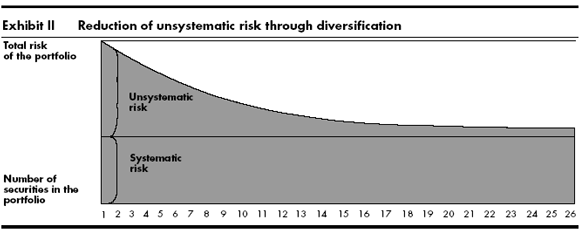
\includegraphics[scale=0.8]{systemic_risk.png}
\caption{Tveganje portfelja glede na število naložb}
\label{risk}
\end{figure}

\subsubsection{Beta koeficient}
%https://corporatefinanceinstitute.com/resources/knowledge/finance/beta-coefficient/		$DONE
Tvegnje je ">izmerjeno"< s tako imenovanim \textbf{beta koeficientom}. Je merilo, ki nam pove,
kako tvegana je naložba v primerjavi s celotnim tržnim tveganjem. Če je beta koeficient neke naložbe
večji od ena, to pomeni, da je naložba nadpovprečno tvegana. Nasprotno, če je beta koeficient 
manjši od ena, to pomeni, da je naložba podpovprečno tvegana. Beta koeficiente za pretekla 
obdobja je mogoče tudi izračunati. Formula ni zapletena. Označimo:
\begin{itemize}
  \item $r_d$ predstavlja donos delnice,
  \item $r_m$ tržne donose in
  \item $\beta_d$ beta koeficient delnice.
\end{itemize}
Potem velja 
$$\beta_d = \frac{cov(r_d, r_m)}{var(r_m)}.$$
Seveda pa se trg neprestano spreminja in stari podatki niso vedno povsem zanesljivi. Žal pa
za prihodnja obdobja ni preproste formule za izračun beta koeficientov. Zato se v praksi 
uporabljajo kar stari podatki, ki so v skrajnem primeru malo ">popravljeni"<, če se v prihodnjem
obdobju pričakuje drastične spremembe stanja na trgu.

%https://pages.stern.nyu.edu/~adamodar/New_Home_Page/datafile/Betas.html			%DONE
\begin{table}[h]
\begin{tabular}{l|c}
\textbf{Industrija}                       & \textbf{Beta} \\ \hline
Banke (regijske)                               & 0,64 \\
Poslovne in potrošniške storitve               & 0,93 \\
Računalniške storitve                          & 1,12 \\
Zdravila (biotehnologija)                      & 0,89 \\
Zdravila (farmacevtska)                        & 0,91 \\
Elektronika                                    & 0,89 \\
Finančne storitve (razen bank in zavarovalnic) & 0,80  \\
Zdravstveni izdelki                            & 0,83 \\
Nafta/plin (produkcija in odkrivanje)          & 1,18 \\
Nepremičninski investicijski skladi            & 1,21 \\
Programska oprema (sistemi in aplikacije)      & 0,91 \\
Maloprodaja (živila)                           & 0,24 \\
Zračni promet                                  & 1,61
\end{tabular}
\caption{Beta koeficienti po sektorjih}
\label{bete}
\end{table}

Tabela \ref{bete} prikazuje beta koeficiente po industrijskih panogah. Sklepamo lahko, da 
je zračni promet najbolj tvegana panoga, na drugi strani spektra pa so podjetja, ki se ukvarjajo 
z maloprodajo živil. Rezultat je precej smiseln, povpraševanje po živilih se načeloma 
ne spreminja veliko. Zračni promet se veliko hitreje razvija, poleg tega pa trenutna
epidemološka slika doda velik vprašaj na prihodnost podjetij v tej industriji. 
Beta koeficienti ostalih industrijskih panog se pravzaprav gibajo blizu $1$. Podatki, iz 
katerih so izračunani beta koeficienti, so bili pridobljeni januarja 2021.


\subsubsection{Formula}
Formula CAPM modela je precej preprosta. Naj bodo:
\begin{itemize}
  \item $r_i$ donos investicije (iskan podatek),
  \item $r_m$ tržni donos,
  \item $r_f$ donos netvegane naložbe (netvegana obrestna mera) in
  \item $\beta_i$ beta koeficient investicije.
\end{itemize}
Potem po CAPM modelu velja sledeča formula:
$$r_i = r_f + \beta_i (r_m - r_f),$$
kjer izraz v oklepaju ($r_m - r_f$) imenujemo tudi \textbf{premija za tveganje}. Iz formule je res
razvidno, da lahko investitorji za večje tveganje (večji beta koeficient) pričakujejo večje donose.
Smiselno je omeniti, da je pričakovane tržne donose in pa tržne donose včasih težko oceniti, zato 
v praksi pogosto namesto njih kot približek vzamemo donose kakšnega indeksa, je pa potrebno 
paziti, da so potem tudi beta koeficienti izračunani glede na ta isti indeks.

\subsubsection{Problemi}
Za korektnost CAPM modela zahtevamo kar nekaj predpostavk, ki v praksi morda niso vedno 
izpolnjene. Tak primer je recimo predpostavka o učinkovitosti trga oz. o hitremu kroženju informacij.
Ta problem je bil v preteklosti bistveno večja težava kot v informacijski dobi, a vseeno obstaja
t.i. \textit{insider trading}, ali trgovanje na podlagi notranjih informacij. Gre za trgovanje, kjer
odločitve o naložbah potekajo delno ali v celoti na podlagi informacij, ki niso dostopne javnosti,
temveč le nekemu zaprtemu krogu. V splošnem je to ilegalno, z izjemo posebnih primerov (npr.
vodilni in zaposleni lahko kupujejo delnice svojega podjetja, čeprav imajo morda več informacij
kot javnost), zadnjo besedo o legalnosti pa ima komisija za borzni nadzor. 

Smiselno je omeniti tudi, da CAPM model predpostavlja, da imajo vsi investitorji enak pogled na 
tveganje. V praksi ne velja niti trditev, da so vsi investitorji nenaklonjeni k tveganu (kljub temu,
da drži za veliko večino, obstajajo izjeme), kaj šele, da bi vsi tveganje obravnavali popolnoma 
enako. Zahtevamo tudi, da so donosi netvegane naložbe konstantni. To je lahko težava, še 
posebej za daljša obdobja, saj se tudi netvegana obrestna mera skozi čas spreminja. 

CAPM model trdi, da so prihodnje vrednosti delnic porazdeljene normalno, kar ne drži nujno.
Kot tudi prej omenjene predpostavke, tudi zadnja v praksi in na resničnem trgu ne drži. Vseeno
pa je model zelo uporaben. Dejstvo je, da tudi če predpostavke niso izpolnjene, so vsaj 
">skoraj izpolnjene"<. Kršitve so bodisi zelo redke, bodisi imajo zelo majhen vpliv na trg. 
Posledično tudi CAPM model ni popoln, vseeno pa so rezultati dovolj natančni, da si lahko 
z njim precej pomagamo. Poleg tega pa je model tudi zelo preprost. To sta tudi glavna vzroka,
da je model še danes v uporabi.


\subsection{Black-Scholesova formula}
%https://en.wikipedia.org/wiki/Black%E2%80%93Scholes_model						%DONE
Black-Scholesov model (poznan tudi pod imenom Black–Scholes–Mertonov model) je model za 
vrednostenje opcijskih pogodb oz. opcij. Ekonomista Fischer Black in Myron Scholes sta leta 
1970 razvila model, ki je po njima dobil ime, zasluge pa lahko pripišemo tudi Robertu C. Mertonu.
Je prva eksplicitna metoda vrednotenja kateregakoli izvedenega 
finančnega instrumenta, v tem primeru opcije. Model predpostavlja, da imajo vrednosti sredstev logaritemsko 
normalno porazdelitev (če je spremenljivka $X$ porazdeljena logaritemsko normalno, je 
$\ln X$ porazdeljen normalno). Model se uporablja izključno za evropske opcije. Razlog za 
to je dejstvo, da ne upošteva možnosti predčasne izvršitve, ki ga kakšni drugi tipi opcij nudijo. 

\subsubsection{Zgodovina}
Leta 1968 sta Black in Scholes demonstrirala, da je mogoče oblikovati tak dinamičen portfelj,
da so njegovi pričakovani donosi vedno enaki nič. Idejo sta dobila iz dela nekaterih matematikov in 
raziskovalcev trga, med drugim tudi že prej omenjenega Louisa Bachelierja. Tako sta ustvarila 
do tveganja nevtralen portfelj. Zaenkrat se to ne sliši še nič kaj obetavno -- in res ni poželo
nobenih uspehov. Ko sta novo znanje uporabila na trgu, sta si naredila precejšnje izgube.
Vzrok je bil v površnosti pri upravljanju s tveganjem (delno tudi zaradi pomanjkanja obstoječih
orodij namenjenim obvladovanju tveganja). 

Nato sta se leta 1970 vrnila v akademsko okolje
in razvila svoj model. Temeljil je na parcialni diferencialni enačbi, ki opisuje gibanje cene
opcije skozi čas. Glavna ideja je, da je z nakupi in prodajami osnovnega sredstva
mogoče popolnoma eliminirati tveganje. Sledi tudi, da obstaja poštena cena opcije, za 
katero sta izpeljala tudi formulo. Leta 1973 je bila formula tudi javno objavljena.
Robert C. Merton je objavil članek v Dnevniku politične ekonomije (angl. \textit{Journal 
of Political Economy}), v katerem razlaga matematično ozadje vrednotenja opcij. Model je
poimenoval kot Black-Scholesov model za vrednotenje opcij in ime je ostalo nespremenjeno
(podobno tudi za Black-Scholesovo formulo, ter Black-Scholesovo enačbo).

\subsubsection{Predpostavke}
%https://www.investopedia.com/terms/b/blackscholes.asp							%DONE
Model je smiseln le pod določenimi pogoji. Zato je pomembno, da navedemo sledeče 
predpostavke.
\begin{itemize}
  \item Opcija je evropska; pomembno je dejstvo, da je izvršitev možna le ob dospetju,
	in ne ob kateremkoli vmesnem času,
  \item osnovno sredstvo ne izplačuje dividend,
  \item trg je učinkovit,
  \item ni transakcijskih stroškov,
  \item tako netvegana obrestna mera kot volatilnost osnovnega sredstva sta znani
	in konstantni skozi celotno obdobje in
  \item donosi osnovnega sredstva so porazdeljeni logaritemsko normalno.
\end{itemize}
Omenimo še, da je predpostavka o ničelnih dividendah kar stroga. Model postane
neuporaben za opcije, katerih osnovno sredstvo izplačuje kakršnekoli dividende. Zato
je model mogoče prilagoditi tako, da deluje tudi za opcije na sredstva, ki izplačujejo
dividende (upoštevati je treba čase in vrednosti izplačil dividend). Tudi omejitev na zgolj
evropske opcije je včasih nadležna, a na srečo obstajajo posplošitve tudi za druge 
tipe opcij, ki nudijo možnost izvršitve pred dospetjem.

\subsubsection{Formula}
Naj bodo:
\begin{itemize}
  \item $N(x) = \frac{1}{\sqrt{2\pi}} \int_{-\infty}{x} e^{-\frac{y^2}{2}} dy$
  \item $T$ čas dospetja,
  \item $S_t$ vrednost instrumenta v času $t$,
  \item $K$ izvršilna cena,
  \item $r$ netvegana obrestna mera in
  \item $\sigma$ standardni odklon.
\end{itemize}
Označimo še
$$d_1 = \frac{\ln (\frac{S_0}{K}) + (r + \frac{\sigma^2}{2})T}{\sigma \sqrt{T}},$$
in pa 
$$d_2 = d_1 -  \sigma T.$$
Potem lahko vrednost nakupne opcije ($C$) izračunamo po naslednji formuli:
\begin{equation}\label{bs1}
C = S_0 N(d_1) - Ke^{-rT}N(d_2),
\end{equation}
vrednost prodajne opcije ($P$) pa prav tako po zelo podobni formuli:
\begin{equation}\label{bs2}
P = Ke^{-rT}N(-d_2) - S_0 N(-d_1).
\end{equation}
Izpeljava oz. dokaz obeh formul pa sta kar precejšen zalogaj, zato jih bom izpustil. Dokazali smo
jo pri predmetu Finančna matematika 1 in dokaz je na voljo v skripti predmeta v petem poglavju
(tam je malce drugačna, saj je razložena v poglavju, ki govori o binomskem modelu, ta pa temelji
na diskretnem času. Zgornja verzija predpostavlja zvezen čas in zvezno obrestovanje).
%Vir do izpeljave???


\section{RiskMetrics in CreditMetrics}
%https://en.wikipedia.org/wiki/J.P._Morgan_%26_Co.							%DONE
%
Ameriška investicijska banka J.P. Morgan je v letih 1992 in 1997 izdala dva notranja 
modela za upravljanje s tveganjem. Imenovala sta se RiskMetrics in CreditMetrics
Temeljila sta na ideji, da je skupno tveganje portfelja
mogoče izmeriti z upoštevanjem tako imenovane tvegane vrednosti (angl. \textit{value
at risk, VaR}). Slednje merilo tveganja je bilo takrat sicer nov koncept, ki pa se je po izidu
prvega izmed modelov zelo hitro globalno razširil. Tvegana vrednost predstavlja največjo
vrednost, ki jo portfelj oz. posledično investitor lahko teoretično izgubi v določenem 
časovnem obdobju, podano z določeno stopnjo zaupanja. Investitorjem omogoča tudi
izračun optimalne količine kapitala potrebne za zaščito svojega portfelja pred izgubami.

\subsection{Merjenje tveganja}
Postopek merjenja tveganja lahko opravimo po korakih in prvi korak je modeliranje trga. 
Model mora biti dovolj specifičen, da lahko naš portfelj ovrednotimo po informacijah 
tega modela. Iz verjetnostne porazdelitve vrednosti portfelja lahko nato ">izmerimo"< 
tvegajne. Ker tveganje samo po sebi seveda nima enote, so se razvila določene mere
tveganja, ki nam povejo veliko koristnih kvantitativnih informacij. 

%https://en.wikipedia.org/wiki/Standard_deviation								%DONE
\subsubsection{Standardni odklon}
Prvo, najpreprostejše in tudi najbolj razširjeno tako merilo je standardni odklon (angl. 
\textit{standard deviation}), ki ga najpogosteje označujemo s $\sigma$. V splošnem 
gre za merilo odstopanja od povprečne oz. pričakovane vrednosti. V normalni porazdelitvi 
poznamo tako imenovano $68-95-99,7$ pravilo (angl. \textit{68--95--99,7 rule}), ki nam
pove, da znotraj intervala $[\mu - \sigma, \mu + \sigma]$ (tu smo z $\mu$ označili 
pričakovano vrednost) nahaja 68\% celotnega vzorca. Na intervalu $[\mu - 2\sigma,
\mu + 2\sigma]$ se nahaja 95\% populacije, in na intervalu $[\mu - 3\sigma, \mu + 3\sigma]$
99,7\% populacije. Daje nam občutek, kako pogosto lahko pričakujemo kako velika
odstopanja od pričakovane vrednosti. 

%mam 3 vire tle													%DONE
\subsubsection{Tvegana vrednost}
Takrat nova mera, ki pa se je do danes že močno razširila, je že prej omenjena
tvegana vrednost. Uporablja se za izračun količine sredstev, ki jo bo potencialno
treba pokriti (v primeru izgub). Tako imenovana $p$ - tvegana vrednost (angl. \textit{p-VaR}) nam 
torej pove največji možen obseg izgub, brez upoštevanja najslabših $1 - p$  
scenarijev. Če ima naložba npr. $95\%$ tvegano vrednost enako en milijon evrov, 
potem obstaja $5\%$ verjetnost, da bo naložba prinesla en milijon evrov izgub ali več.
Drugače povedano, z verjetnostjo $95\%$ trdimo, da bodo izgube manjše od enega
milijona evrov.

\subsubsection{Pričakovani izpad}
%https://en.wikipedia.org/wiki/Expected_shortfall								%DONE
Naslednje merilo je pričakovani izpad. Gre za podobno merilo prejšnjemu, glavna
razlika pa je ta, da se pričakovani izpad osredotoča na najhujše možne scenarije.
Osredotoča se na spodnji del verjetnostne porazdelitve oz. na obliko porazdelitvene
krivulje v skrajnem spodnjem delu. Pogosto mu rečemo tudi povprečna ali pogojna
tvegana vrednost. Pričakovani izpad nivoja $q$ lahko definiramo na sledeč način:
$$ES_q(X) = -\frac{1}{q} \int_0^q VaR_p(X) dp.$$

Pričakovani izpad nivoja $q$ nam poda pričakovane izgube, pod 
pogojem, da se zgodi eden izmed $q$ najslabših možnih izidov. Najpogosteje se 
v praksi računa pričakovani izpad nivoja $5\%$. 

\subsubsection{Mejna tvegana vrednost}
Poznamo tudi mejno tvegano vrednost (angl. \textit{Marginal Value at Risk}), ki
nam pove, koliko posamezna naložba prispeva k tvegani vrednosti celotnega portfelja.
Uporabjla se predvsem pri ocenjevanju doprinosa posamezne naložbe k skupnemu
tveganju portfelja, po tem ko dodamo to naložbo. Izračun je precej preprost; mejna
tvegana vrednost naložbe je enaka razliki med tvegano vrednostjo celotnega 
portfelja, vključno s to naložbo, ter tvegano vrednostjo celotnega portfelja brez
dodatne naložbe.

\subsubsection{Prirastek tveganju}
Najlažje je prirastek tveganju razložen kot neka občutljivost na spremembo velikosti pozicije.
Predstavlja tveganje, ki nastane kot posledica spremembe velikosti pozicije oz. 
obsega naložbe. Tudi za tovrstno tveganje se uporabljajo (prilagojena)
zgoraj našteta merila in so tudi pokrita v RiskMetrics. 


\subsection{Koherentna mera tveganja}
Ker obstaja veliko načinov kako definirati oz. ovrednotiti tveganje, je smiselno 
definirati nekaj lastnosti, ki so zelo priročne za mere tveganja. 
%https://en.wikipedia.org/wiki/Coherent_risk_measure							%DONE
%https://bankaslovenije.blob.core.windows.net/uploaded/O%20nas%2FNagrade%20BS%2FKmet.pdf		%DONE
\begin{definicija}[Koherentna mera tveganja]
	Naj bo $\mathcal{L}$ prostor omejenih realnih slučajnih spremenljivk,
	definiranih na nekem verjetnostnem prostoru, in $\rho: \mathcal{L} \to 
	\mathbb{R} \cup \{\infty\}$ preslikava. Potem je $\rho$ koherentna mera
	tveganja, če zanjo veljajo naslednje lastnosti:
	\begin{enumerate}
		\item $\forall X,Y \in \mathcal{L}: X \leq Y \Rightarrow \rho(X) \leq \rho(Y)$ (monotonost)
		\item $\forall X,Y \in \mathcal{L}: \rho(X+ Y) \leq \rho(X) + \rho(Y)$ (subaditivnost)
		\item $\forall \alpha > 0, \forall X \in \mathcal{L} \Rightarrow \rho(\alpha X) = \alpha \rho(X)$ (pozitivna homogenost)
		\item $\forall t \in \mathbb{R}, \forall X \in \mathcal{L}: \rho(X + t) = \rho(X) + t$ (translacijska invarianca)
	\end{enumerate}
\end{definicija}

\begin{opomba}
	V definiciji bi lahko subaditivnost in pozitivno homogenost izpustili, in namesto 
	njiju zahtevali konveksnost:
	\begin{itemize}
		\item $X,Y \in \mathcal{L}, \lambda \in [0, 1] \Rightarrow \rho(\lambda X + (1-\lambda) Y) \leq \lambda \rho(X) + (1 - \lambda) \rho(Y)$
	\end{itemize}
\end{opomba}

%https://bankaslovenije.blob.core.windows.net/uploaded/O%20nas%2FNagrade%20BS%2FKmet.pdf		%DONE (isti)

Če $X$ predstavlja portfeljsko izgubo, potem lahko $\rho(X)$ interpretiramo kot
potreben kapital za zavarovanje pred izgubo $X$. Intuitivno so vse zahtevane 
lastnosti koherentne mere tveganja zelo preproste in zelo pomembne. Monotonost
zahtevamo, ker želimo, da za večje potencialne izgube zahtevamo več kapitala za 
kritje. 
Vemo, da je z razpršitvijo naložbe mogoče odpraviti specifično tveganje. Subaditivnost
predstavlja točno ta pojav; skupno tveganje razpršene naložbe ($X + Y$) bo kvečjemu
enako vsoti tveganj posameznih naložb $X$ in $Y$.
Homogenost nam pove, da sorazmerno povečanje oz. zmanjšanje vseh naložb za
faktor $\lambda$ poveča tudi zahtevani kapital za kritje tveganja za isti faktor. Zadnjo 
lastnost pa si lahko razlagamo na sledeč način. Če portfelju dodamo v  naprej znano 
konstantno izgubo ali dobiček $t$, potem se tudi skupno tvegnaje poveča ali zmnajša za
natanko za $t$.

\begin{trditev}
Tvegana vrednost (\textit{VaR}) \textbf{ni} koherentna mera tveganja.
\end{trditev}

\begin{proof}
Za tvegano vrednost je mogoče dokazati tri izmed štirih zahtevanih lastnosti.
Mi bomo poiskali protiprimer, ki dokazuje, da tvegana vrednost \textbf{ni}
subaditivna.
Naj bosta $X_1$ in $X_2$ dva neodvisna portfelja, oba porazdeljena Bernoullijevo, torej  $X_1 \sim X_2 \sim Ber(p)$, 
za $p = 0.009$. Z verjetnostjo $p$ ima portfelj popolno oz. $100\%$ izgubo, 
na drugi strani pa z verjetnostjo $1-p$ portfelj nima nobene izgube. 
Ker je verjetnost izgube v obeh portfeljih manjša od $1\%$, velja:
$$VaR_{99\%}(X_1) = VaR_{99\%}(X_2) = 0.$$
Poglejmo zdaj unijo (vsoto) obeh portfeljev. Če želimo, da so izgube enake $0$,
morata oba portfelja imeti izgube enake $0$. Verjetnost tega dogodka je enaka:
$$P(X_1 + X_2 = 0) = P(X_1 = 0)P(X_2 = 0) = (1-p)^2 = 0,991^2 = 0,982081.$$
Ker je verjetnost tega dogodka manjša od $99\%$, ne moremo z verjetnostjo $99\%$
trditi, da bodo izgube enake $0$. Sledi:
$$VaR_{99\%}(X_1 + X_2) > 0$$
in nato
$$VaR_{99\%}(X_1 + X_2) > VaR_{99\%}(X_1) + VaR_{99\%}(X_2),$$
torej smo poiskali protiprimer, ki dokazuje, da tvegana vrednost ni subaditivna
in posledično ni koherentna mera tveganja.
\end{proof}

Dejstvo, da tvegana vrednost ni subaditivna je nerodna reč, saj v določenih 
primerih odsvetuje diverzifikacijo, ki pa je splošno znana kot učinkovita strategija, 
saj (vsaj delno) eliminira specifično tveganje. V primeru, ko so izgube porazdeljene 
normalno in je vrednost portfelja linearna funkcija vrednosti sredstev, pa je v 
resnici tudi tvegana vrednost koherentna. Pričakovani izpad je koherentna 
mera tveganja.


\subsection{Modeliranje trga}
Kot že omenjeno, je postopek merjenja tveganja lahko opravljen po korakih. Modeliranje trga je morda
najpomembnejši korak. RiskMetrics opisuje
tri različne pristope modeliranja dejavnikov, ki oblikujejo finančne trge:

\subsubsection{Kovariančni pristop}
Najpreprostejši izmed treh. Temelji na ideji, da
obstajajo kovariance med različnimi dejavniki, ki vplivajo na trg, pa tudi 
med donosi različnih sredstev. Z uporabo kovarianc oz. kovariančnih 
matrik je mogoče izračunati varianco portfelja. 


\subsubsection{Zgodovinska simulacija}
Predpostavimo, da ima trg le končno mnogo
možnih sprememb, ki jih lahko pridobimo iz preteklih dogodkov. Ugotovitve 
nato po potrebi prilagodimo in vzorce prenesemo na trenutne razmere na 
trgu. Metoda je zelo preprosta, ni pa pretirano prilagodljiva. V primeru 
drastičnih sprememb na trgu bi se znalo zgoditi, da bi model potreboval kar
nekaj časa, da bi se na novo stanje na trgu dobro ">privadil"<. Zaradi tega 
v takem primeru pogosto pripelje do zavajajočih rezultatov.


\subsubsection{Monte Carlo simulacija}
Metoda predpostavlja, da logaritem izkupičkov
naložbe sledi normalni porazdelitvi, rizični dejavniki pa so porazdeljeni 
(večrazsežno) normalno. S simulacijo nato generiramo ogromno količino 
naključnih scenarijev, ob vsaki ponovitvi pa si zabeležimo
profit ali izgubo. Iz tega lahko potem dobimo vzorčno porazdelitev
profita oz. izgube naložbe, kar pa nam omogoča nadaljno računanje 
različnih meril tveganja. 

Pogosto se v matematiki srečamo z zahtevnimi problemi. Čeprav imamo dandanes
na voljo zelo zmogljive računalnike za pomoč pri reševanju zahtevnih računskih
vprašanj, včasih tudi to ni dovolj, ali pa tak pristop ne bi bil dovolj hiter oz.
učinkovit. Najbolj pomembna lastnost Monte Carlo simulacije je dejstvo, da 
uporablja naključja. S tem se izogne računskemu reševanju zahtevnih problemov,
namesto tega pa na preprost način ">s poskušanjem"< reši te probleme. 
Seveda z uporabo takega pristopa rezultat ne bo tako natančen, kot če bi
se reševanja lotili na direkten način. Je pa z večanjem števila poskusov možno
doseči vedno večjo natančnost in zelo pogosto je simulacija z ogromnim 
številom ponovitev že zelo natančna (pogosto celo z zanemarljivo napako), 
hkrati pa še vedno mnogo hitrejša od tradicionalnega postopka.


%https://en.wikipedia.org/wiki/Financial_regulation								%DONE
\section{Regulacija}
Zaradi različnih oblik tveganja lahko pri poslovanju pride do raznovrstnih težav. 
Zato so regulacije zelo pomembne. S pojmom regulacija najpogosteje označujemo
razne oblike nadzora, pravil ali smernic. Finančna regulacija je oblika 
regulacije, ki zavezuje finančne inštitucije in od njih zahteva, da sledijo določenim
smernicam pri poslovanju in se držijo določenih zahtev. Nadzor lahko opravljajo 
tako vladne kot nevladne organizacije. Skozi čas so imele regulacije velik vpliv na 
trg, med drugim tudi na količino različnih produktov na voljo. Cilji finančne 
regulacije so naslednji:
\begin{itemize}
  \item ohranjanje zaupanja v trg,
  \item zaščita in izboljšanje stabilnosti finančnega sistema in
  \item zagotavljanje primerne količine zaščite strank in tržnih udeležencev.
\end{itemize}

Določene organizacije, zadolžene za regulacijo trgov, 
imajo moč posegati v poslovanje. Njihova naloga je spremljati dogajanje in
v primeru kršitev ali spornih aktivnosti ukrepati. Obstajajo različni finančni
regulatorni sistemi.
\begin{itemize}
  \item \textbf{Borzni nadzor}: Menjalni akti zagotavljajo, da se trgovanje na 
	borzah izvaja pravilno. Najpomembnejši del je proces oblikovanja cen, 
	izvedba in poravnava poslov ter neposredno in učinkovito spremljanje trga.
  \item \textbf{Nadzor podjetij, ki kotirajo na borzi}: Regulatorji zagotavljajo, da
	podjetja upoštevajo zadane smernice. Podjetja, ki kotirajo na borzi, morajo
	redno izdajati finančna poročila, da obvestijo javnost (in predvsem svoje
	investitorje) in jim dajo na voljo informacije o trenutnem stanju podjetja.
	Po potrebi morajo izdajati tudi posebna obvestila. Cilj je investitorjem 
	zagotoviti dostop do zadostnih in nujno potrebnih informacij, da lahko
	sprejemajo informirane odločitve glede svojih investicij.
  \item \textbf{Nadzor investicijskega managementa}: Nadzor upravljanja sredstev
	in akti o naložbah minimizirajo trenje na trgu.
  \item \textbf{Nadzor bank in ponudnikov finančnih storitev}: Bančni akti določajo 
	pravila za banke, ki jih morajo upoštevati že ob ustanavljanju, pa tudi pri 
	poslovanju. Pravila so zasnovana tako, da preprečijo nezaželen razvoj 
	dogodkov, ki bi potencialno zmotil delovanje in stabilnost bančnega sistema.
	Tako pomagajo zagotoviti močan, učinkovit in stabilen bančni sistem.
\end{itemize}


\subsection{Bančni nadzor}
Banke so ena izmed finančnih inštitucij, s katero ima opravka največje število oseb.
Od podjetij in pravnih oseb pa tudi do fizičnih oseb, tudi če se ne ukvarjajo s  
financami. V Združenih državah Amerike, imajo komercialne banke v povprečju 
kar za $3,1$ milijarde ameriških dolarjev depozitov (vodilne štiri banke sicer močno
dvigajo to povprečje, a vseeno). Denarja, ki ga stranke prinesejo na banko pa ne 
hranijo pri roki ali v kakšnem sefu, kot mnogi zmotno mislijo. 

Denar od depozitov lahko banke uporabijo pri svojem poslovanju. S tem se pojavijo 
različne vrste tveganja: kaj se zgodi v primeru, ko stranke želijo množično 
dvigovati velike vsote denarja, banka pa nima dovolj likvidnih sredstev, saj jih je 
vložila v nek projekt? Kaj se zgodi, če banka ta denar celo izgubi npr. v slabem poslu?

Seveda banke pri poslovanju srečujejo tudi druga tveganja. Da jih omejijo, 
obstajajo določene regulacije, ki jih določi vlada oz. pristojna vladna organizacija, 
ali pa jih določa kakšna tretja organizacija in jim banke sledijo prostovoljno, tudi 
če to ni zakonsko določeno. 

%https://en.wikipedia.org/wiki/Basel_Committee_on_Banking_Supervision					%DONE
\subsubsection{Bazelski odbor za bančni nadzor}
Čeprav po zakonu Bazelski odbor za bančni nadzor (angl. \textit{Basel Committee 
on Banking Supervision}) nima moči zahtevati upoštevanja standardov s strani bank, 
le-te (vsaj večina) vseeno sledijo smernicam. Gre za mednarodni organ, ki razvija 
standarde za regulacijo bank. Sestavlja ga 45 centralnih bank in drugih regulatornih
organov iz 28 različnih pristojnosti. Ustanovile so ga centralne banke članic tako 
imenovanega G-10 (angl. \textit{Group of 10}) leta 1974. Članice so si prizadevale
zgraditi mednaroden finančni sistem. Tako kot drugi odbori, ima tudi Bazelski odbor 
za bančni nadzor svoje ureditve upravljanja in agende, ki jih vodijo guvernerji 
centralnih bank iz ">skupine desetih"<.

\subsubsection{Basel I}
%https://www.investopedia.com/terms/b/basel_i.asp								%DONE
%https://www.investopedia.com/terms/b/baselii.asp									%DONE
Prvi sistem regulacij izdan s strani Bazelskega odbora za bančni nadzor je prvi
bazelski sporazum (angl. \textit{Basel I}). Izšel je leta 1988 in bil uveljavljen 
leta 1992. Leto kasneje je odbor potrdil, da vse države G10 oz. njihove banke 
izpolnjujejo zahteve sporazuma. Basel I zahteva, da morajo banke v vsakem 
trenutku imeti na voljo dovolj kapitala, da pokrijejo vsaj $8\%$ njihovega profila
tveganja. Če ima banka torej tehtano vrednost tveganih sredstev enako $100$ milijonov
evrov, mora imeti pri roki vsaj $8$ milijonov evrov kapitala ali drugih oblik likvidnih sredstev. Tehtana vrednost 
temelji na klasifikaciji sredstev po tveganju  v pet različnih kategorij: $0\%$, $10\%$, $20\%$, 
$50\%$ in $100\%$. Vsa sredstva so klasificirana v eno izmed kategorij na 
podlagi narave dolžnika. Po mnenju mnogih je bil ta set regulacij preveč 
poenostavljen, imel pa je še 2 naslednika.

\subsubsection{Basel II}
%https://whatis.techtarget.com/definition/Basel-II									%DONE
Naslednji komplet regulacij je bil drugi bazelski sporazum (angl. \textit{Basel II}). 
Oblikovan je bil leta 2004 in sprejet 2 leti kasneje. Do leta 2008 je bil že precej dobro 
implementiran, čeprav so ga nekatere banke preskočile in še danes sledijo 
prvemu bazelskemu sporazumu z dodatnimi dopolnili, ki pa izvirajo iz tretjega. 
Sporazum naj bi imel tri stebre:
\begin{itemize}
  \item minimalne kapitalske zahteve,
  \item regulativni nadzor in
  \item tržna disciplina,
\end{itemize}
s spremembami oz. novostmi v primerjavi z njegovim predhodnikom predvsem 
v zadnjih dveh stebrih. 

Ohranja zahtevo po imetju $8\%$ profila tveganja v obliki kapitala. Regulatorni 
kapital deli v tri sloje (v primerjavi z dvema nivojema prvega bazelskega sporazuma).
Višja stopnja predstavlja manj podrejen kapital. Sporazum vključuje tudi predpisano 
strukturo regulatornega kapitala po omenjenih stopnjah. Prva stopnja (angl. \textit{Tier 
1 capital}) vključuje lastniški kapital, rezerve, zadržani dobiček, ter nekatere 
inovativne kapitalske instrumente, kapital druge (angl. \textit{Tier 2 capital}) in 
tretje stopnje (angl. \textit{Tier 3 capital}) pa vključujeta tudi določene hibridne 
instrumente in posojila različnih ročnosti.

\subsubsection{Basel III}
%https://en.wikipedia.org/wiki/Basel_III										%DONE
Tretji bazelski sporazum (angl. \textit{Basel III}) je tretji in trenutno zadnji 
implementiran komplet regulacij izdan s strani bazelskega odbora za bančni 
nadzor. Sprejet je bil novembra 2010, implementacija pa je bila predvidena med 
leti 2013 in 2015, a je bila večkrat prestavljena in v resnici sistem še danes ni 
dobro implementiran. Nastal je predvsem kot odgovor na napake oz. pomanjkljivosti 
v njegovem predhodniku, Basel II, ki so se izkazale med finančno krizo leta 2008. 

V tem sporazumu se je prvič pojavila zahteva, da banke vzdržujejo minimalen nivo 
razmerja finančnega vzvoda (angl. \textit{leverage ratio}). Izračunamo ga lahko 
kot razmerje med kapitalom prve stopnje in skupno izpostavljenostjo. Basel III 
zahteva, da banke vzdržujejo razmerje nad $3\%$. Od zasnove se je zahteva 
tudi malce spremenila oz. povišala in varira po svetu, v Evropski Uniji pa morajo banke le javno 
objaviti svoje razmerje finančnega vzvoda, minimalen nivo pa ni prepdisan. 

\subsubsection{Basel IV}
%https://en.wikipedia.org/wiki/Basel_IV										%DONE
Četrti bazelski sporazum (angl. \textit{Basel IV}) je četrti komplet regulacij zasnovan 
s strani bazelskega odbora za bančni nadzor. Sprejet je bil leta 2017, implementacija 
pa je predvidena do januarja 2023. Gre le za dopolnitev pravil, ki jih narekuje njegov 
predhodnik, zato ga v Veliki Britaniji imenujejo kar \textit{Basel 3.1}.


\subsection{Borzni nadzor}
%https://en.wikipedia.org/wiki/List_of_stock_exchanges								%DONE
%https://en.wikipedia.org/wiki/U.S._Securities_and_Exchange_Commission					%DONE
Glavne naloge borznega nadzora so sledeče:
\begin{itemize}
  \item regulacija odnosov tržnih udeležencev,
  \item zaščita pravic in interesov investitorjev,
  \item nadzor nad profesionalnimi udeleženci trga, samo-regulatornimi organizacijami
	in drugimi entitetami, katerih dejavnosti na trgu se izvajajo na podlagi 
	določenih licenc, dovoljenj ali drugih pogodb.
\end{itemize}
Različne organizacije nadzirajo različne borze. Morda najpomembnejša tovrstna 
organizacija je Ameriška komisija za vrednostne papirje in borzo (angl. \textit{
U.S. Securities and Exchange Commission, SEC}), saj je zadolžena za nadzor dveh 
daleč največjih borz na svetu. To sta newyorška borza (angl. \textit{New York Stock 
Exchange, NYSE}) in Nasdaq, ki sta daleč na prvem mestu tako po tržni kapitalizaciji, 
kot tudi obsegu trgovanja. 

\subsubsection{Ameriška komisija za vrednostne papirje in borzo}
Ustanovljena je bila 6. junija 1934 kot odgovor na zlom newyorške borze leta 1929 
(angl. \textit{Wall Street Crash of 1929}). Zaradi zlorab in goljufij na finančnih trgih 
sta bila kot del programa New Deal sprejeta zakon o vrednostnih papirjih iz 1933 (angl 
\textit{Securities Act of 1933}) in zakon o prodaji vrednostnih papirjev iz 1934 (angl. \textit{ Securities 
Exchange Act of 1934}), z njima pa je bila uveljavljena avtoriteta Ameriške 
komisije za vrednostne papirje in borzo. 

Na vrhu ima pet komisarjev, ki jih določi predsednik. Največ trije lahko pripadajo isti 
politični stranki. Ima pet divizij: 
\begin{itemize}
  \item \textbf{Podjetniške finance}: nadzoruje javna podjetja in registracijo 
	transakcij, kot so npr. združitve.
%https://en.wikipedia.org/wiki/Financial_Industry_Regulatory_Authority						%DONE
  \item \textbf{Trg in trgovanje}: oddelek nadzoruje samo-regulatorne organizacije, 
	kot sta ameriški regulator finančne industrije (angl \textit{Financial Industry 
	Regulatory Authority, FINRA}) in lokalni regulator trga vrednostnih papirjev 
	(angl. \textit{Municipal Securities Rulemaking Board, MSRB}). Oddelek interperita 
	predlagane spremembe predpisov in spremlja dogajanje v industriji, večino 
	izvrševanja pa opravi FINRA.
  \item \textbf{Investicijski nadzor}: divizija nadzoruje reigstrirana investicijska 
	podjetja in investicijske svetovalce (npr. vzajemne sklade) na podlagi 
	večih različnih aktov. Med drugim tudi pomagajo javnosti pri interpretaciji 
	zakonov in regulacij ter svetujejo komisiji glede prilagoditev na nove 
	razmere
  \item \textbf{Izvršba}: ta oddelek preiskuje kršitve zakonov in predpisov, na 
	podlagi tega pa po potrebi vlaga tožbe proti domnevnim kršiteljem. Gre za 
	največji oddelek komiteja, tako po številu zaposlenih kot po proračunu. 
  \item \textbf{Analiza ekonomije in tveganja}: glavna naloga je vključitev finančne 
	ekonomije in analize podatkov v osnovno nalogo komisije. Oddelek je vključen 
	v vse dejavnosti komisije, vključno z oblikovanjem pravil in politik ter izvrševanjem.
\end{itemize}


\section{Strukturirane finance}
%https://www.investopedia.com/terms/s/structuredfinance.asp							%DONE
Skozi čas so bila podjetja vedno bolj aktivna pri poslovanju, pojavljali pa so se novi 
instrumenti. Zato so podjetja potrebovala vedno bolj specifične oblike financiranja. Pojavile 
so se \textbf{strukturirane finance} (angl. \textit{strucutred finance}). Gre za bolj 
zakomplicirane finančne instrumente, ki so predvsem namenjeni večjim finančnim 
inštitucijam ali podjetjem. Od sredine osemdesetih let so postale zelo popularne. 
Podjetja in inštitucije se zanje odločajo zato, ker imajo pri svojem poslovanju zelo 
specifične potrebe po financiranju, tradicionalna ponudba instrumentov pa ne nudi 
takega spektra izplačil kot strukturirane finance. 

Najpopularnejši primeri so zadolžnice, zavarovane z dolgom (angl. \textit{collateralized 
debt obligations, CDOs}),	sintetični finančni instrumenti, zadolžnice, zavarovane z 
obveznicami (angl. \textit{collateralized bond obligations, CBOs})
in pa sindicirana posojila. Tradicionalni posojilodajalci v splošnem ne ponujajo nobenega 
izmed naštetih instrumentov. Namenjeni so predvsem upravljanju s tveganjem, 
koristni pa so bili tudi pri razvoju finančnih trgov za kompleksne nastajajoče trge.

\subsection{Pogodbe na razlike}
%https://www.investopedia.com/terms/c/contractfordifferences.asp						%DONE
Zelo preprost izveden finančni insturment so pogodbe na razlike (angl. \textit{
Contract for Differences, CFD}). Kupec instrumenta verjame, da bo cena osnovnega 
sredstva zrasla. Če ima prav, ob zaprtju pozicije prejme razliko v vrednosti 
osnovnega sredstva od trenutka odprtja pozicije do trenutka zaprtja kot profit. 
V nasportnem primeru bo ta razlika negativna in predstavlja investitorjevo izgubo. 

Instrument je postal zelo popularen, saj omogoča velike donose za zelo majhen 
začetni vložek (izdajalci najpogosteje zahtevajo zelo majhen delež celotne vrednosti 
osnovnega sredstva, pogosto okoli $5\%$). S tem pa seveda pride tudi veliko 
tveganje. Že sam po sebi je instrument ekstremno volatilen, za povrh pa še niso 
dobro regulirani, zato je težko oceniti kredibilnost izdajatelja. V Združenih državah 
Amerike so zato celo prepovedani.

\subsection{Zadolžnice, zavarovane z dolgom}
%https://www.investopedia.com/terms/c/cdo.asp									%DONE
%https://en.wikipedia.org/wiki/Collateralized_debt_obligation							%DONE
Čeprav so se do 2003/2004 uporabljali le redko, so CDO-ji tekom nepremičninskega 
mehurčka v ZDA postali zelo popularni. Izdajalci teh instrumentov so začeli kot 
zavarovanje sprejemati tudi hipotekarno zavarovane vrednostne papirje, kar je 
povzročilo povečanje povpraševanja po teh instrumentih. Za financiranje CDO-jev 
so se v letu 2006 začeli uporabljati bolj tvegani instrumenti. Posojila na 
trgu so postala vedno bolj tvegana, sčasoma pa je to pripeljalo tudi do finančne 
krize. Več o tem v poglavju \ref{kriza}, za zdaj pa si poglejmo strukturo CDO-ja.	 

\subsubsection{Struktura}
Instrument ima precej zapleteno strukturo. Razdeljen je v sekcije, imenovane tudi 
">rezine"< oz. ">tranše"< (angl. \textit{tranches}). Delijo se glede na varnost oz. tveganje, 
višja sekcija pomeni nižje tveganje. Investitorji so potem razdeljeni v te rezine. 

Manager zadolžnic, zavarovanih z dolgom, predhodno izbere sredstva, ki bodo 
vključena v CDO-jih. Izplačila teh sredstev se nato zbirajo in izplačajo investitorjem. 
Vsako sredstvo ima različna izplačila in tudi različno tveganje.

Zaradi tveganja neplačila določenih instrumentov, ki financirajo zadolžnice, zavarovane 
z dolgom, obstaja možnost, da nekateri investitorji ne bodo poplačani. Izplačila prvi 
prejmejo investitorji v višjih razredih, nazadnje pa tisti v nižjih razredih. Zaradi 
nižjega tveganja investitorji v višjih rezinah prejmejo nižje donose, tisti v nižjih 
sekcijah pa zaradi višjega tveganja neplačila pričakujejo višje donose. Za lažje 
razumeavnje je na sliki \ref{cdo_structure} prikazana shema CDO-jev. 

\begin{figure}[h]
\centerline{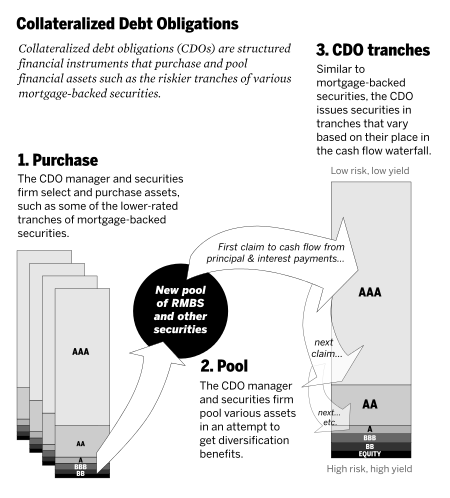
\includegraphics[scale=0.5]{CDO_structure.png}}
\caption{Struktura zadolžnic, zavarovanih z dolgom}
\label{cdo_structure}
\end{figure}

Poglejmo si še nekaj specifičnih tipov zadolžnic, zavarovanih z dolgom.

\subsection{Zadolžnice, zavarovane z obveznicami}
%https://www.investopedia.com/terms/c/cbo.asp									%DONE
Strukturiran na podoben način kot zadolžnice, zavarovane z dolgom, je tudi ta 
instrument izdan po tranšah in poplačuje investitorje po enakem vrstnem redu 
kot pri ostalih CDO-jih. Zelo podobne so zadolžnice, zavarovane s hipoteko. V resnici 
gre za tip CDO-ja, le da je kriterij izbire instrumentov bolj strog. Če so vsi instrumenti 
obveznice, potem gre za CBO, sicer pa za CDO.

Ideja je sledeča: obveznice z nižjimi ocenami so bolj tveganje, a prinašajo višje 
donose. Listinenje obveznic različnih izdajalcev, četudi so vse obveznice ocenjene 
z nizko oceno in spadajo v ">junk"< razred, pa zaradi diverzifikacije postane 
veliko manj tvegana naložba. Tako lahko iz samih tveganih in slabo ocenjenih 
obveznic ustvarijo instrument, ki pa je ocenjen z višjo oceno. V praksi jih večinoma 
uvrščajo v investicijski razred kljub temu, da morda v listinenju ni niti ene obveznice, 
ki spada v isti razred.

\subsection{Zadolžnice, zavarovane z hipotekami}
%https://www.investopedia.com/terms/c/cmo.asp									%DONE
Na enak način delujejo tudi zadolžnice, zavarovane s hipotekami, edina razlika je 
seveda ta, da se za financiraje uporablja hipoteke namesto obveznic. Struktura 
instrumenta je sicer zelo podobna. Pred finančno krizo leta 2008 se je količina 
teh instrumentov močno povečala, postali so zelo popularni, nato pa so po 
poku mehurčka skoraj da povsem izginili. Spet gre za tip CDO-ja, kjer so vključeni 
le instrumenti istega tipa (v tem primeru hipoteke). Če bi vključevale še kakšen 
drug instrument, potem pa bi šlo preprosto za CDO.

\subsection{Zamenjava kreditnih tveganj}
%https://smartasset.com/investing/credit-default-swap								%DONE
%https://www.investopedia.com/terms/c/creditdefaultswap.asp							%DONE
Dogovor med upnikom in tretjo osebo, kjer tretja oseba prevzame upnikovo tveganje 
neplačila, imenujemo zamenjava kreditnih tveganj (angl. \textit{Credit Default Swap, CDS}). 
Včasih se uporablja tudi izraz zamenjava kreditnih neplalčil.
Seveda je upnik dolžan plačati premijo. S tem instrumentom se efektivno zavaruje 
pred neplačilom, saj v primeru neplačila dolg poravna tretja oseba, s katero je upnik 
sklenil dogovor. Treba pa je omeniti, da tveganje ni povsem eliminirano, saj še 
vedno lahko pride tudi do neplačila s strani izdajatelja zamenjave. 

Popularnost teh instrumentov je bila na vrhuncu med finančno krizo leta 2008, 
poleg tega pa je privedla do enega od glavnih vzrokov za krizo. Kar nekaj 
finančnih inštitucij, ki so izdajale te zamenjave, namreč niso poplačale dolgov.

\subsection{Sintetični CDO}
%https://www.investopedia.com/terms/s/syntheticcdo.asp								%DONE
Malo bolj moderna in napredna verzija CDO-jev so sintetični CDO-ji. (angl. \textit{
Synthetic CDOs}). Znani so tudi kot zadolžnice, zavarovane s sintetičnimi instrumenti 
(angl. \textit{Collateralized synthetic obligations, CSOs}). Struktura je podobna 
klasičnim CDO-jem z eno ključno razliko: 
namesto obveznic, hipotek, in podobnih sredstev, so v sintetičnih CDO-jih zbrani 
izvedeni finančni instrumenti, kot so zamenjave kreditnih neplačil, opcije in drugi. 
Zato lahko nudijo ekstremno visoke donose.

\subsection{CDO drugega reda}
Spet zelo podoben instrument klasičnemu CDO-ju, le da namesto obveznic, 
hipotek in podobnih sredstev, vključuje kar druge CDO-je. Izdajajo ga primarno 
banke. Izdajateljem, ki imajo v lasti zadolžnice, zavarovane z dolgom, dovolijo, 
da svoje obveznosti in kreditno tveganje naprej prodajo in se tako zavarujejo. 
Podobno kot ostali obravnavani instrumenti, so tudi CDO-ji drugega reda postali 
popularni tik pred finančno krizo leta 2008, potem pa se je trg sesul.

Na podoben način so definirani tudi CDO-ji višjega reda. Pogosto jim rečemo 
kar CDO-ji tretjega reda (angl. \textit{CDO cubed}). Vključujejo druge CDO-je, 
lahko pa tudi CDO-je drugega ali višjega reda.

%https://www.investopedia.com/ask/answers/09/bond-rating.asp 		Slika/tabela za bond ratings		%DONE


\section{Finančna kriza 2008}
\label{kriza}
Napake na področju upravljanja s tveganjem zagotovo niso bile edini vzrok za finančno 
krizo leta 2008, so pa prav gotovo imele pomembno vlogo. V nadaljevanju si bomo 
pogledali nekatere izmed površnosti oz. napak na področju upravljanja s tveganjem, 
ki so bile pogoste pred oz. med finančno krizo.


\subsection{Površnost in pomanjkanje informacij}
Prvi dve napaki sta bili površnost in pomanjkanje informacij. Mnoge banke in predvsem 
nepremičninski posredniki niso imeli ustrezne spodbude, da bi bili pozorni in spremljali 
tveganja posojilojemalcev oz. strank. Vzrok za to je dejstvo, da so pogodbe zelo redko 
vključevale pogodbene klavzule v primeru moralnega hazarda. Posledično 
inštitucije niso imele ustrezne motivacije, da bi dosledno skrbele za tveganja svojih 
strank.

Zaradi podobnega vzroka je prišlo tudi do pomanjkanja informacij ali celo napačnih 
informacij. Finančni produkti so ocenjeni glede na njihovo donosnot in tveganje. 
Tipično višje (boljše) ocene pomenijo nižjo donosnost, a hkrati nižje tveganje. 
Spodnja tabela prikazuje ocene instrumentov glede na njihovo oceno tveganja, 	
razvršča pa jih tudi v dva razreda, investicijski razred (angl \textit{investment 
grade}) in tvegane obveznice (angl. \textit{junk bonds}).

\begin{table}[h]
\begin{tabular}{c|c|c|c}
\textbf{Moody's} & \textbf{Standard \& Poor's} & \textbf{Razred}      & \textbf{Tveganje} \\ \hline
Aaa              & AAA                         & investicijski razred & najnižje          \\
Aa               & AA                          & investicijski razred & nizko             \\
A                & A                           & investicijski razred & nizko             \\
Baa              & BBB                         & investicijski razred & srednje           \\
Ba               & BB                          & junk                 & visoko            \\
B                & B                           & junk                 & visoko            \\
Caa, Ca, C       & CCC, CC, C                  & junk                 & najvišje          \\
/                & D                           & junk                 & neplačilo        
\end{tabular}
\caption{\label{ocene}Ocene finančnih produktov}
\end{table}

Kot lahko vidimo v tabeli, so instrumenti z oceno BBB najnižje ocenjeni instrumenti, 
ki še vedno spadajo v investicijski razred. Poplačila npr. obveznic so bila lahko 
uporabljena tudi kot zavarovanje v nekih drugih, strukturiranih instrumentih. 
Standard, ki so ga taki dogovori zahtevali, da se obveznica lahko uporabi kot 
zavarovanje, je najmanj ocena BBB (torej instrument investicijskega razreda). 

Z uporabo dodatnih jamstev prek zamenjav kreditnih tveganj pa so uporabljali 
obveznice standarda BB kot obveznice investicijskega razreda, 
čeprav v resnici niso bile. Tako so preveč tvegane instrumente uporabljali pri 
CDO-jih in drugih kompliciranih izvedenih finančnih instrumentih, čeprav jih v 
resnici nebi smeli, saj ne ustrezajo standardom.

\subsection{Ocene strukturiranih produktov}
Naslednja težava ima v resnici zelo podoben rezultat prejšnjemu primeru, le da 
je vzrok skrit drugje. Omenjene ocene vrednostnih papirjev so zelo pomembe 
za profitabilnost. Med drugim ocena odloča o tem, ali se instrument lahko uporabi 
za financiranje ali ne. Zaradi nenatančnih ocen, so lahko (tako kot v prejšnji 
točki) uporabljali instrumente, ki so bili preveč tvegani, za financiranje v drugih 
strukturiranih instrumentih. 

Treba pa je omeniti, da je bilo zaradi povečanega števila novih instrumentov, 
hkrati pa pomanjkanja podatkov in predvsem modelov za vrednotenje teh 
instrumentov, težko oceniti njihova tveganja. 

\subsection{Regulacija strukturiranih financ}
Zadnja težava se nanaša primarno na banke in zavarovalnice. Kot že omenjeno, 
je takratni sistem regulacij, Basel II, narekoval količino kapitala potrebne za 
kritje različnih profilov tveganja. Instrumenti z različnimi ocenami so bili 
zato obravnavani drugače, to pa je pomenilo, da so bile za te inštitucije 
papirji z najboljšo (AAA) oceno odlična izbira.

Za izdajatelje produktov je postalo zelo pomembno, da pridobijo kar se da 
dobro oceno. To je povzročalo pritisk na bonitetne agencije. Rezultat je 
bil neskladnost ocen. Odličen primer so bile zakladne menice. Ponujale so 
najnižje donose, torej bi morale biti ">najmanj tvegan"< instrument, 
vendar pa (sodeč po ocenah) niso bile. Na trgu so bili tudi papirji, ki so 
ponujali višji donos, hkrati pa naj bi bili manj tvegani.

\subsection{Hipotekarni vrednostni papirji in zadolžnice, zavarovane z dolgom}
Glavni razlog za krizo leta 2008 pa so bile zadolžnice, zavarovane z dolgom, in 
hipotekarni vrednostni papirji (angl. \textit{Mortgage backed securities}). Slednji 
so instrumenti, podobni obveznicam, 
sestavljeni iz stanovanjskih posojil. Izplačujejo podobna izplačila kot dradicionalne 
obveznice (kupone). Oba instrumenta sta bila glavni vir financiranja takratnega 
nepremičninskega balončka (angl. \textit{housing bubble}). 

Vse zgoraj naštete težave so bile opazne pri CDO-jih in hipotekarnih vrednostnih 
papirjih. Piko na i je dodal padec vrednosti osnovnih sredstev teh izvedenih finančnih 
instrumentov, zaradi česar so CDO-ji in hipotekarni vrednostni papirji prav tako izgubili 
velik del vrednosti. To je mnogim podjetjem in inštitucijam povzročilo ogromne izgube. 
Več milijonov lastnikov stanovanj ni poravnalo svojih obveznosti, zato se je porušil 
trg CDO-jev, za najslabšo naložbo pa so se izkazali CMO-ji, saj je ogromen delež 
investitorjev ostal nepoplačan. 

\begin{figure}[h]

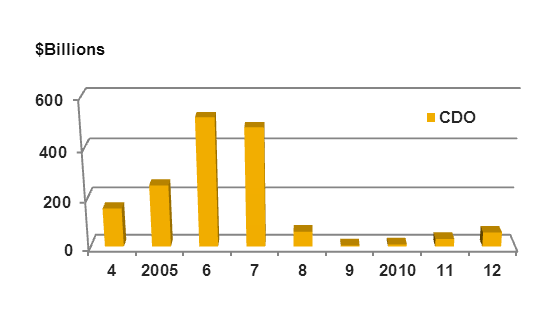
\includegraphics[scale=0.8]{CDO.png}
\caption{Obseg CDO-jev po letih}
\label{graf_CDO}
\end{figure}

Graf na sliki \ref{graf_CDO} prikazuje obseg CDO-jev v posameznih letih, v obdobju pred 
in po finančni krizi leta 2008. Vidimo, da se je obseg močno povečal pred krizo, 
nato pa nenadoma skoraj povsem upadel. Instrument je namreč zelo zanimiv, 
zelo zahtevno pa je oceniti njegovo tveganje, kar pa je bil eden od glavnih 
razlogov za finančno krizo.





% slovar
\section*{Slovar strokovnih izrazov}

\geslo{bull spread}{bikov korak (strategija)}

\geslo{coherent risk measure}{koherentna mera tveganja}

\geslo{collateralized debt obligations}{zadolžnice, zavarovane z dolgom}

\geslo{contract for differences}{pogodba na razlike}

\geslo{correlation matrix}{korelacijska matrika}

\geslo{credit default swap}{zamenjava kreditnih tveganj}

\geslo{derivative}{izvedeni finančni instrument}

\geslo{dynamic portfolio}{dinamični portfelj}

\geslo{expected shortfall}{pričakovani primanjkljaj}

\geslo{future}{terminska pogodba}

\geslo{incremental risk}{prirastek k tveganju}

\geslo{investment grade}{investicijski razred}

\geslo{junk bonds}{tvegane obveznice}

\geslo{leverage ratio}{razmerje finančnega vzvoda}

\geslo{marginal value at risk}{mejna tvegana vrednost}

\geslo{mortgage-backed securities}{hipotekarno zavarovani vrednostni papirji}

\geslo{option}{opcija}

\geslo{over the counter (OTC)}{na prostem trgu}

\geslo{protective put}{zaščitna prodaja}

\geslo{risk}{tveganje}

\geslo{risk management}{upravljanje s tveganjem}

\geslo{risk measure}{mera tveganja}

\geslo{security}{vrednostni papir}

\geslo{settlement date}{datum poravnave}

\geslo{standard deviation}{standardni odklon}

\geslo{strike}{\textbf{$\sim$ rate} izvršilna obrestna mera; \textbf{$\sim$ price} izvršilna cena}

\geslo{structured finance}{strukturirane finance}

\geslo{subprime mortgage}{tvegane hipoteke}

\geslo{swap}{zamenjava}

\geslo{underlying}{osnovno sredstvo}

\geslo{value at risk}{tvegana vrednost}


% seznam uporabljene literature
\begin{thebibliography}{99}

\bibitem{main}
G.~Dionne, \emph{Risk management: History, definition and critique}, 6.~9.~2010; dostopno tudi na
\url{http://www.fmf.uni-lj.si/~globevnik/skripta.pdf}.

\bibitem{history1}
A.~Rhodes, \emph{A Brief Summary of the Long History of Risk Management}, [ogled 12.~7.~2021], dostopno na \url{
https://www.ventivtech.com/blog/a-brief-summary-of-the-long-history-of-risk-management}.

\bibitem{wiki_bachelier}
\emph{Louis Bachelier}, v: Wikipedia: The Free Encyclopedia, [ogled 12.~7.~2021], dostopno na \url{https://en.wikipedia.org/wiki/Louis_Bachelier}.

\bibitem{wiki_brownian_motion}
\emph{Brownian motion}, v: Wikipedia: The Free Encyclopedia, [ogled 12.~7.~2021], dostopno na \url{https://en.wikipedia.org/wiki/Brownian_motion}.

\bibitem{Quote_b_motion}
R.~W.~Dimand, \emph{The case of Brownian motion: a note on Bachelier's contribution}, v: The British Journal for the History of Science,\ \textbf{Volume 26, Issue 2}, junij\ 1993, str.\ 233-234, dostopno tudi na \url{https://www.cambridge.org/core/journals/british-journal-for-the-history-of-science/article/abs/case-of-brownian-motion-a-note-on-bacheliers-contribution/EFCA1863B23ACF2339CCF9E6C26EB659}.

\bibitem{wiki_jof}
\emph{The Journal of Finance}, v: Wikipedia: The Free Encyclopedia, [ogled 12.~7.~2021], dostopno na \url{https://en.wikipedia.org/wiki/The_Journal_of_Finance}.

\bibitem{wiki_afa}
\emph{American Finance Association}, v: Wikipedia: The Free Encyclopedia, [ogled 12.~7.~2021], dostopno na \url{https://en.wikipedia.org/wiki/American_Finance_Association}.

\bibitem{aria}
[ogled 12.~7.~2021], dostopno na \url{https://www.aria.org/about-aria/}.

\bibitem{wiki_jri}
\emph{Journal of Risk and Insurance}, v: Wikipedia: The Free Encyclopedia, [ogled 13.~7.~2021], dostopno na \url{https://en.wikipedia.org/wiki/Journal_of_Risk_and_Insurance}.

\bibitem{inv_future}
\emph{Futures Contract}, v: Investopedia, [ogled 13.~7.~2021], dostopno na \url{https://www.investopedia.com/terms/f/futurescontract.asp}.

\bibitem{inv_swap}
\emph{Swap}, v: Investopedia, [ogled 13.~7.~2021], dostopno na \url{https://www.investopedia.com/terms/s/swap.asp}.

\bibitem{wiki_option}
\emph{Option (finance)}, v: Wikipedia: The Free Encyclopedia, [ogled 13.~7.~2021], dostopno na \url{https://en.wikipedia.org/wiki/Option_(finance)}.

\bibitem{inv_option}
\emph{Swap}, v: Investopedia, [ogled 13.~7.~2021], dostopno na \url{https://www.investopedia.com/terms/s/swap.asp}.

\bibitem{inv_protective_put}
\emph{Protective Put}, v: Investopedia, [ogled 15.~7.~2021], dostopno na \url{https://www.investopedia.com/terms/p/protective-put.asp}.

\bibitem{inv_bull}
\emph{Bull Spread}, v: Investopedia, [ogled 15.~7.~2021], dostopno na \url{https://www.investopedia.com/terms/b/bullspread.asp}.

\bibitem{inv_capm}
\emph{Capital Asset Pricing Model (CAPM)}, v: Investopedia, [ogled 15.~7.~2021], dostopno na \url{https://www.investopedia.com/terms/c/capm.asp}.

\bibitem{capm_xy}
D.~W.~Mullins Jr.,\emph{Does the Capital Asset Pricing Model Work?}, v: Harvard Business Review, [ogled 19.~7.~2021], dostopno na \url{https://hbr.org/1982/01/does-the-capital-asset-pricing-model-work}.
%Zgorn je tud vir slike

\bibitem{beta}
\emph{What is the Beta Coefficient?}, [ogled 19.~7.~2021], dostopno na \url{https://corporatefinanceinstitute.com/resources/knowledge/finance/beta-coefficient/}.

\bibitem{beta_table}
\emph{Betas by Sector (US)}, [ogled 19.~7.~2021], dostopno na \url{https://pages.stern.nyu.edu/~adamodar/New_Home_Page/datafile/Betas.html}.

\bibitem{wiki_bs}
\emph{Black–Scholes model}, v: Wikipedia: The Free Encyclopedia, [ogled 20.~7.~2021], dostopno na \url{https://en.wikipedia.org/wiki/Black\%E2\%80\%93Scholes_model}.

\bibitem{inv_bs}
\emph{Black-Scholes Model}, v: Investopedia, [ogled 20.~7.~2021], dostopno na \url{https://www.investopedia.com/terms/b/blackscholes.asp}.

\bibitem{wiki_JP_Morgan}
\emph{J.P. Morgan \& Co.}, v: Wikipedia: The Free Encyclopedia, [ogled 28.~7.~2021], dostopno na \url{https://en.wikipedia.org/wiki/J.P._Morgan_\%26_Co.}.

\bibitem{wiki_deviation}
\emph{Standard Deviation}, v: Wikipedia: The Free Encyclopedia, [ogled 28.~7.~2021], dostopno na \url{https://en.wikipedia.org/wiki/Standard_deviation}.

\bibitem{inv_var}
\emph{What Is Value at Risk (VaR)?}, v: Investopedia, [ogled 28.~7.~2021], dostopno na \url{https://www.investopedia.com/terms/v/var.asp}.

\bibitem{inv_var2}
\emph{An Introduction to Value at Risk (VAR)}, v: Investopedia, [ogled 28.~7.~2021], dostopno na \url{https://www.investopedia.com/articles/04/092904.asp}.

\bibitem{wiki_var}
\emph{Value at risk}, v: Wikipedia: The Free Encyclopedia, [ogled 28.~7.~2021], dostopno na \url{https://en.wikipedia.org/wiki/Value_at_risk}.

\bibitem{wiki_es}
\emph{Expected shortfall}, v: Wikipedia: The Free Encyclopedia, [ogled 28.~7.~2021], dostopno na \url{https://en.wikipedia.org/wiki/Expected_shortfall}.

\bibitem{wiki_coherent}
\emph{Coherent risk measure}, v: Wikipedia: The Free Encyclopedia, [ogled 1.~8.~2021], dostopno na \url{https://en.wikipedia.org/wiki/Coherent_risk_measure}.

\bibitem{diploma}
A.~Kmet, \emph{Modeliranje kreditnih tveganj}, diplomsko delo, Fakulteta za matematiko in fiziko, Univerza v Ljubljani, 2005, dostopno tudi na \url{https://bankaslovenije.blob.core.windows.net/uploaded/O\%20nas\%2FNagrade\%20BS\%2FKmet.pdf}

\bibitem{wiki_reg}
\emph{Financial regulation}, v: Wikipedia: The Free Encyclopedia, [ogled 2.~8.~2021], dostopno na \url{https://en.wikipedia.org/wiki/Financial_regulation}.

\bibitem{wiki_bcbs}
\emph{Basel Committee on Banking Supervision}, v: Wikipedia: The Free Encyclopedia, [ogled 2.~8.~2021], dostopno na \url{https://en.wikipedia.org/wiki/Basel_Committee_on_Banking_Supervision}.

\bibitem{inv_basel1}
\emph{Basel I}, v: Investopedia, [ogled 2.~8.~2021], dostopno na \url{https://www.investopedia.com/terms/b/basel_i.asp}.

\bibitem{inv_basel2}
\emph{Basel II}, v: Investopedia, [ogled 2.~8.~2021], dostopno na \url{https://www.investopedia.com/terms/b/baselii.asp}.

\bibitem{basel2}
\emph{Basel II}, [ogled 2.~8.~2021], dostopno na \url{https://whatis.techtarget.com/definition/Basel-II}.

\bibitem{wiki_basel3}
\emph{Basel III}, v: Wikipedia: The Free Encyclopedia, [ogled 2.~8.~2021], dostopno na \url{https://en.wikipedia.org/wiki/Basel_III}.

\bibitem{wiki_basel4}
\emph{Basel IV}, v: Wikipedia: The Free Encyclopedia, [ogled 2.~8.~2021], dostopno na \url{https://en.wikipedia.org/wiki/Basel_IV}.

\bibitem{wiki_exchanges}
\emph{List of stock exchanges}, v: Wikipedia: The Free Encyclopedia, [ogled 3.~8.~2021], dostopno na \url{https://en.wikipedia.org/wiki/List_of_stock_exchanges}.

\bibitem{wiki_sec}
\emph{U.S. Securities and Exchange Commission}, v: Wikipedia: The Free Encyclopedia, [ogled 3.~8.~2021], dostopno na \url{https://en.wikipedia.org/wiki/U.S._Securities_and_Exchange_Commission}.

\bibitem{wiki_finra}
\emph{Financial Industry Regulatory Authority}, v: Wikipedia: The Free Encyclopedia, [ogled 3.~8.~2021], dostopno na \url{https://en.wikipedia.org/wiki/Financial_Industry_Regulatory_Authority}.

\bibitem{inv_sf}
\emph{Structured Finance}, v: Investopedia, [ogled 3.~8.~2021], dostopno na \url{https://www.investopedia.com/terms/s/structuredfinance.asp}.

\bibitem{inv_cfd}
\emph{What Is a Contract for Differences (CFD)?}, v: Investopedia, [ogled 3.~8.~2021], dostopno na \url{https://www.investopedia.com/terms/c/contractfordifferences.asp}.

\bibitem{inv_cdo}
\emph{Collateralized Debt Obligation (CDO)}, v: Investopedia, [ogled 3.~8.~2021], dostopno na \url{https://www.investopedia.com/terms/c/cdo.asp}.

\bibitem{wiki_cdo}
\emph{Collateralized debt obligation}, v: Wikipedia: The Free Encyclopedia, [ogled 3.~8.~2021], dostopno na \url{https://en.wikipedia.org/wiki/Collateralized_debt_obligation}.

\bibitem{inv_cbo}
\emph{Collateralized Bons Obligation (CBO)}, v: Investopedia, [ogled 3.~8.~2021], dostopno na \url{https://www.investopedia.com/terms/c/cbo.asp}.

\bibitem{inv_cmo}
\emph{Collateralized Mortgage Obligation (CMO)}, v: Investopedia, [ogled 3.~8.~2021], dostopno na \url{https://www.investopedia.com/terms/c/cmo.asp}.

\bibitem{cds}
\emph{How Does a Credit Default Swap Work?}, v: smartasset, [ogled 4.~8.~2021], dostopno na \url{https://smartasset.com/investing/credit-default-swap}.

\bibitem{inv_cds}
\emph{Credit Default Swap (CDS)}, v: Investopedia, [ogled 4.~8.~2021], dostopno na \url{https://www.investopedia.com/terms/c/creditdefaultswap.asp}.

\bibitem{inv_syn_cdo}
\emph{Synthetic Collateralized Debt Obligation (CDO)}, v: Investopedia, [ogled 4.~8.~2021], dostopno na \url{https://www.investopedia.com/terms/s/syntheticcdo.asp}.

\bibitem{inv_ratings}
\emph{How Are Bonds Rated?}, v: Investopedia, [ogled 4.~8.~2021], dostopno na \url{https://www.investopedia.com/ask/answers/09/bond-rating.asp}.

\bibitem{inv_mbs}
\emph{Mortgage-Backed Security (MBS)}, v: Investopedia, [ogled 6.~8.~2021], dostopno na \url{https://www.investopedia.com/terms/m/mbs.asp}.

\bibitem{inv_cdo_kriza}
\emph{Were Collateralized Debt Obligations Responsible for the Financial Crisis?}, v: Investopedia, [ogled 6.~8.~2021], dostopno na \url{https://www.investopedia.com/ask/answers/032315/were-collateralized-debt-obligations-cdo-responsible-2008-financial-crisis.asp}.

\bibitem{wiki_kriza}
\emph{Subprime mortgage crisis}, v: Wikipedia: The Free Encyclopedia, [ogled 6.~8.~2021], dostopno na \url{https://en.wikipedia.org/wiki/Subprime_mortgage_crisis}.

\end{thebibliography}


%%\nocite{*}
%%\bibliographystyle{plain}
%%\bibliography{literatura}


\end{document}

